%%%%%%%%%%%%%%%%%%%%%%%%%%%
%DIF LATEXDIFF DIFFERENCE FILE
%DIF DEL main_original.tex   Fri Nov 13 12:10:08 2026
%DIF ADD main.tex            Fri Nov 13 12:10:08 2026
% IEEE Submission Dashboard - https://ieee.atyponrex.com/submission/dashboard
%%%%%%%%%%%%%%%%%%%%%%%%%%%

% IEEE Transactions on human--machine systems
% https://ieeexplore.ieee.org/xpl/mostRecentIssue.jsp?punumber=6221037

%---------------------------------------------------------------------
% \documentclass[10pt,journal,compsoc]{IEEEtran}
% \documentclass[lettersize,journal]{IEEEtran}
% \documentclass[letterpaper,journal]{IEEEtran}
\documentclass[journal]{IEEEtran}
% ==== Core packages (normalized) ====

% How to hide statements:
%   - To enable  tags: \iftrue  and \fi
%   - To disable tags: \iffalse and \fi
% How to turn-on (or turn-off) page number:
%   - To turn-on  the page number: {plain}
%   - To turn-off the page number: {empty}
% Usage (Syntax):
%   \documentstyle[twocolumn]{article}
%   \pagestyle{empty}
%    ...
%   \maketitle
%   \thispagestyle{empty}

% How to print the page number at each page
\pagestyle{empty}

\usepackage[T1]{fontenc}
\usepackage[utf8]{inputenc}
\usepackage{microtype}
\usepackage{amsmath,amssymb}
\usepackage{amsthm}  % theorem 환경을 사용하기 위한 필수 패키지
%\usepackage{amsmath}
%\usepackage{amssymb}
\usepackage{makecell}
%\usepackage{amsmath,amsfonts,amssymb,mathtools}
%\usepackage{amsthm}
\usepackage{graphicx}
\usepackage{booktabs}
\usepackage{siunitx}
\usepackage{xspace}
\usepackage{pifont}
% Checkmark / Xmark symbols
\newcommand{\cmark}{\ding{51}}
\newcommand{\xmark}{\ding{55}}

\usepackage{listings}
\usepackage{xcolor}
\usepackage{xurl}
\usepackage{url}

% Hyperlinks to content
% \usepackage[linktocpage=true]{hyperref}
% \usepackage{hyperref}
% \usepackage[nameinlink]{cleveref}
% \usepackage[hidelinks]{hyperref}
\usepackage[colorlinks=true,linkcolor=blue,citecolor=blue,urlcolor=black]{hyperref}

\usepackage{cleveref}
%\usepackage{amsmath,amsfonts}
% \usepackage{algorithmic}
\usepackage{algorithm}
\usepackage{array}
\usepackage[caption=false,font=normalsize,labelfont=sf,textfont=sf]{subfig}
\usepackage{textcomp}
\usepackage{stfloats}
\usepackage{verbatim}
\usepackage{cite}
%\hyphenation{op-tical net-works semi-conduc-tor IEEE-Xplore}
%\usepackage{amssymb,amsmath,amsthm,mathtools}
%\usepackage{hyphenat}

%% ------------- ORC ID Template: Start ----------------------
% https://tex.stackexchange.com/questions/498688/orcid-in-latex-file-of-ieee-trans-in-a-customized-position

\usepackage{scalerel}
\usepackage{tikz}
\usetikzlibrary{svg.path}

\definecolor{orcidlogocol}{HTML}{A6CE39}
\tikzset{
orcidlogo/.pic={
\fill[orcidlogocol] svg{M256,128c0,70.7-57.3,128-128,128C57.3,256,0,198.7,0,128C0,57.3,57.3,0,128,0C198.7,0,256,57.3,256,128z};
\fill[white] svg{M86.3,186.2H70.9V79.1h15.4v48.4V186.2z}
svg{M108.9,79.1h41.6c39.6,0,57,28.3,57,53.6c0,27.5-21.5,53.6-56.8,53.6h-41.8V79.1z M124.3,172.4h24.5c34.9,0,42.9-26.5,42.9-39.7c0-21.5-13.7-39.7-43.7-39.7h-23.7V172.4z}
svg{M88.7,56.8c0,5.5-4.5,10.1-10.1,10.1c-5.6,0-10.1-4.6-10.1-10.1c0-5.6,4.5-10.1,10.1-10.1C84.2,46.7,88.7,51.3,88.7,56.8z};
}
}

\newcommand\orcidicon[1]{\href{https://orcid.org/#1}{\mbox{\scalerel*{

\begin{tikzpicture}[yscale=-1,transform shape]
    \pic{orcidlogo};
\end{tikzpicture}
}{|}}}}

%% ------------- ORC ID Template: End ----------------------

\providecommand{\cmark}{\ding{51}}
\providecommand{\xmark}{\ding{55}}
\providecommand{\etal}{\textit{et al.}\xspace}
\DeclareMathOperator{\E}{\mathbb{E}}
\DeclareMathOperator{\Var}{\mathrm{Var}}

\theoremstyle{plain}
\newtheorem{theorem}{Theorem}[section]
\newtheorem{lemma}{Lemma}[section]
\newtheorem{corollary}{Corollary}[section]
\lstdefinelanguage{json}{
basicstyle=\ttfamily\small,
numbers=left,
numberstyle=\tiny,
stepnumber=1,
showstringspaces=false,
breaklines=true
}
\lstset{frame=single}
% === End patch ===

\IEEEoverridecommandlockouts

%####################################################### Geunsik Area ###########

\usepackage{algorithm}
\usepackage{algpseudocode}

% LaTeX에서 유니코드(①, ② 등)를 직접 사용
\usepackage{pifont}

% theorem, algorithm 가독성위해 디자인 개선
\usepackage[most]{tcolorbox}
\tcbuselibrary{listings}

%% To keep strictly tuned whitespace rules among sections (e.g., section, subsection, and subsubsection)
%% for decreasing or increasing the vertical space between sections
\usepackage{titlesec}
\titlespacing*{\section}{0.70pt}{0.50\baselineskip}{0.20\baselineskip}
\titlespacing*{\subsection}{0.70pt}{0.50\baselineskip}{0.20\baselineskip}
\titlespacing*{\subsubsection}{0.70pt}{0.50\baselineskip}{0.20\baselineskip}

%% Reduce vertical space (padding) after figure (a big effect)
%% Warning: "Text page 7 contains only floats."
%% https://www.reddit.com/r/LaTeX/comments/b4mipa/how_to_decrease_space_between_paragraph_and/
\setlength{\textfloatsep}{0.70pt}
\setlength{\abovecaptionskip}{0.70pt}
\setlength{\belowcaptionskip}{0.70pt}

\theoremstyle{definition}
\newtheorem{definition}{Definition}[section]
\urlstyle{tt}

\newcommand{\Lninetyfive}{L_{95}}
\newcommand{\Jain}{\mathcal{J}}
\providecommand{\cmark}{\ding{51}}
\providecommand{\xmark}{\ding{55}}

% JSON language for listings
\lstdefinelanguage{json}{
basicstyle=\ttfamily\small,
numbers=left, numberstyle=\tiny, stepnumber=1,
showstringspaces=false,
breaklines=true
}

% Listings setup (handles code blocks and JSON/diff-like listings)
\lstset{basicstyle=\ttfamily\small, breaklines=true, columns=fullflexible, showstringspaces=false}

% Minimal JSON language for listings
\lstdefinelanguage{json}{
basicstyle=\ttfamily\small,
showstringspaces=false,
morestring=[b]",
morecomment=[l]{//},
literate=
*{0}{{{\color{black}0}}}{1}
{1}{{{\color{black}1}}}{1}
{2}{{{\color{black}2}}}{1}
{3}{{{\color{black}3}}}{1}
{4}{{{\color{black}4}}}{1}
{5}{{{\color{black}5}}}{1}
{6}{{{\color{black}6}}}{1}
{7}{{{\color{black}7}}}{1}
{8}{{{\color{black}8}}}{1}
{9}{{{\color{black}9}}}{1}
{:}{{{\color{black}{:}}}}{1}
{,}{{{\color{black}{,}}}}{1}
{"}{{{\color{black}{"}}}}{1}
}
%DIF PREAMBLE EXTENSION ADDED BY LATEXDIFF
%DIF CFONT PREAMBLE %DIF PREAMBLE
\RequirePackage{color}\definecolor{RED}{rgb}{1,0,0}\definecolor{BLUE}{rgb}{0,0,1} %DIF PREAMBLE
\DeclareOldFontCommand{\sf}{\normalfont\sffamily}{\mathsf} %DIF PREAMBLE
\providecommand{\DIFaddtex}[1]{{\protect\color{blue} \sf #1}} %DIF PREAMBLE
\providecommand{\DIFdeltex}[1]{{\protect\color{red} \scriptsize #1}} %DIF PREAMBLE
%DIF SAFE PREAMBLE %DIF PREAMBLE
\providecommand{\DIFaddbegin}{} %DIF PREAMBLE
\providecommand{\DIFaddend}{} %DIF PREAMBLE
\providecommand{\DIFdelbegin}{} %DIF PREAMBLE
\providecommand{\DIFdelend}{} %DIF PREAMBLE
\providecommand{\DIFmodbegin}{} %DIF PREAMBLE
\providecommand{\DIFmodend}{} %DIF PREAMBLE
%DIF FLOATSAFE PREAMBLE %DIF PREAMBLE
\providecommand{\DIFaddFL}[1]{\DIFadd{#1}} %DIF PREAMBLE
\providecommand{\DIFdelFL}[1]{\DIFdel{#1}} %DIF PREAMBLE
\providecommand{\DIFaddbeginFL}{} %DIF PREAMBLE
\providecommand{\DIFaddendFL}{} %DIF PREAMBLE
\providecommand{\DIFdelbeginFL}{} %DIF PREAMBLE
\providecommand{\DIFdelendFL}{} %DIF PREAMBLE
%DIF HYPERREF PREAMBLE %DIF PREAMBLE
\providecommand{\DIFadd}[1]{\texorpdfstring{\DIFaddtex{#1}}{#1}} %DIF PREAMBLE
\providecommand{\DIFdel}[1]{\texorpdfstring{\DIFdeltex{#1}}{}} %DIF PREAMBLE
\newcommand{\DIFscaledelfig}{0.5}
%DIF HIGHLIGHTGRAPHICS PREAMBLE %DIF PREAMBLE
\RequirePackage{settobox} %DIF PREAMBLE
\RequirePackage{letltxmacro} %DIF PREAMBLE
\newsavebox{\DIFdelgraphicsbox} %DIF PREAMBLE
\newlength{\DIFdelgraphicswidth} %DIF PREAMBLE
\newlength{\DIFdelgraphicsheight} %DIF PREAMBLE
% store original definition of \includegraphics %DIF PREAMBLE
\LetLtxMacro{\DIFOincludegraphics}{\includegraphics} %DIF PREAMBLE
\newcommand{\DIFaddincludegraphics}[2][]{{\color{blue}\fbox{\DIFOincludegraphics[#1]{#2}}}} %DIF PREAMBLE
\newcommand{\DIFdelincludegraphics}[2][]{% %DIF PREAMBLE
\sbox{\DIFdelgraphicsbox}{\DIFOincludegraphics[#1]{#2}}% %DIF PREAMBLE
\settoboxwidth{\DIFdelgraphicswidth}{\DIFdelgraphicsbox} %DIF PREAMBLE
\settoboxtotalheight{\DIFdelgraphicsheight}{\DIFdelgraphicsbox} %DIF PREAMBLE
\scalebox{\DIFscaledelfig}{% %DIF PREAMBLE
\parbox[b]{\DIFdelgraphicswidth}{\usebox{\DIFdelgraphicsbox}\\[-\baselineskip] \rule{\DIFdelgraphicswidth}{0em}}\llap{\resizebox{\DIFdelgraphicswidth}{\DIFdelgraphicsheight}{% %DIF PREAMBLE
\setlength{\unitlength}{\DIFdelgraphicswidth}% %DIF PREAMBLE
\begin{picture}(1,1)% %DIF PREAMBLE
\thicklines\linethickness{2pt} %DIF PREAMBLE
{\color[rgb]{1,0,0}\put(0,0){\framebox(1,1){}}}% %DIF PREAMBLE
{\color[rgb]{1,0,0}\put(0,0){\line( 1,1){1}}}% %DIF PREAMBLE
{\color[rgb]{1,0,0}\put(0,1){\line(1,-1){1}}}% %DIF PREAMBLE
\end{picture}% %DIF PREAMBLE
}\hspace*{3pt}}} %DIF PREAMBLE
} %DIF PREAMBLE
\LetLtxMacro{\DIFOaddbegin}{\DIFaddbegin} %DIF PREAMBLE
\LetLtxMacro{\DIFOaddend}{\DIFaddend} %DIF PREAMBLE
\LetLtxMacro{\DIFOdelbegin}{\DIFdelbegin} %DIF PREAMBLE
\LetLtxMacro{\DIFOdelend}{\DIFdelend} %DIF PREAMBLE
\DeclareRobustCommand{\DIFaddbegin}{\DIFOaddbegin \let\includegraphics\DIFaddincludegraphics} %DIF PREAMBLE
\DeclareRobustCommand{\DIFaddend}{\DIFOaddend \let\includegraphics\DIFOincludegraphics} %DIF PREAMBLE
\DeclareRobustCommand{\DIFdelbegin}{\DIFOdelbegin \let\includegraphics\DIFdelincludegraphics} %DIF PREAMBLE
\DeclareRobustCommand{\DIFdelend}{\DIFOaddend \let\includegraphics\DIFOincludegraphics} %DIF PREAMBLE
\LetLtxMacro{\DIFOaddbeginFL}{\DIFaddbeginFL} %DIF PREAMBLE
\LetLtxMacro{\DIFOaddendFL}{\DIFaddendFL} %DIF PREAMBLE
\LetLtxMacro{\DIFOdelbeginFL}{\DIFdelbeginFL} %DIF PREAMBLE
\LetLtxMacro{\DIFOdelendFL}{\DIFdelendFL} %DIF PREAMBLE
\DeclareRobustCommand{\DIFaddbeginFL}{\DIFOaddbeginFL \let\includegraphics\DIFaddincludegraphics} %DIF PREAMBLE
\DeclareRobustCommand{\DIFaddendFL}{\DIFOaddendFL \let\includegraphics\DIFOincludegraphics} %DIF PREAMBLE
\DeclareRobustCommand{\DIFdelbeginFL}{\DIFOdelbeginFL \let\includegraphics\DIFdelincludegraphics} %DIF PREAMBLE
\DeclareRobustCommand{\DIFdelendFL}{\DIFOaddendFL \let\includegraphics\DIFOincludegraphics} %DIF PREAMBLE
%DIF COLORLISTINGS PREAMBLE %DIF PREAMBLE
\RequirePackage{listings} %DIF PREAMBLE
\RequirePackage{color} %DIF PREAMBLE
\lstdefinelanguage{DIFcode}{ %DIF PREAMBLE
%DIF DIFCODE_CFONT %DIF PREAMBLE
  moredelim=[il][\color{red}\scriptsize]{\%DIF\ <\ }, %DIF PREAMBLE
  moredelim=[il][\color{blue}\sffamily]{\%DIF\ >\ } %DIF PREAMBLE
} %DIF PREAMBLE
\lstdefinestyle{DIFverbatimstyle}{ %DIF PREAMBLE
	language=DIFcode, %DIF PREAMBLE
	basicstyle=\ttfamily, %DIF PREAMBLE
	columns=fullflexible, %DIF PREAMBLE
	keepspaces=true %DIF PREAMBLE
} %DIF PREAMBLE
\lstnewenvironment{DIFverbatim}{\lstset{style=DIFverbatimstyle}}{} %DIF PREAMBLE
\lstnewenvironment{DIFverbatim*}{\lstset{style=DIFverbatimstyle,showspaces=true}}{} %DIF PREAMBLE
%DIF END PREAMBLE EXTENSION ADDED BY LATEXDIFF

\begin{document}

    %----------------------------------------\input{./001-title}

    \title{From Alerts to Actions: A Human--AI Decision System for Reliable Action Execution Under Disaster Risk}

    %---------------------------------- \input{./003-author}

    \author{

    % for ORC-ID
    \IEEEauthorblockN{
    Geunsik Lim$^{\textsuperscript{\orcidicon{0000-0003-1845-7132}}}$
    }


    \thanks{G. Lim is with the Department of Electrical and Computer Engineering, Sungkyunkwan University, 2066, Seobu-ro, Jangan-gu, Suwon 16419, South Korea (e-mail: leemgs@g.skku.edu). }

    }

    % The paper headers
    % \markboth{Journal of \LaTeX\ Class Files,~Vol.~14, No.~8, August~2015}%
    % {Shell \MakeLowercase{\textit{et al.}}: Bare Demo of IEEEtran.cls for IEEE Transactions on Magnetics Journals}

    \DIFdelbegin %DIFDELCMD < \markboth{IEEE Transactions on Consumer Electronics, Vol. 1, No. 1, May 2020}{G. Lim \MakeLowercase{\text
%DIFDELCMD <     {et al.}}: Thread Evolution Kit for Optimizing Thread Operations on IoT Devices}
%DIFDELCMD < %%%
\DIFdelend \DIFaddbegin \markboth{IEEE Transactions on Human-Machine Systems}{Lim: From Alerts to Actions: A Human--AI Decision System Under Disaster Risk}
\DIFaddend 

    % make the title area
    \maketitle

    \thispagestyle{empty}%

    % -----------------------------\input{./005-abstract}
    \begin{abstract}
        \DIFdelbegin \DIFdel{Decision systems involving human and AI are being used in critical situations where inappropriate actions on the part of the human could result in }\DIFdelend \DIFaddbegin \DIFadd{Human--AI decision systems are increasingly used in situations where an inappropriate or delayed human action can have }\DIFaddend serious consequences. \DIFdelbegin \DIFdel{Even though there has been an improvement }\DIFdelend \DIFaddbegin \DIFadd{Improvements }\DIFaddend in the predictive \DIFdelbegin \DIFdel{capabilities of AI , it does notautomatically translate to appropriate actions on the part of the human . The focus of this paper is to understand how the structure of a human--AI decision systemaffects action execution, trust, and cognitive workload in uncertain situations.
        We introduce a new concept for human--AI decision system design: \emph{Action-Centered Human--AI Decision Framework (ACHDF)}, which focuses on action execution rather than on the performance of the algorithm.
        Our mixed-method evaluation strategy using controlled user studies }\DIFdelend \DIFaddbegin \DIFadd{accuracy of AI do not, by themselves, translate into appropriate human action. Drawing on the joint cognitive systems perspective, which evaluates the human and the machine as a single system, we present the \emph{Action-Centered Human--AI Decision Framework (ACHDF)}. ACHDF instantiates uncertainty-aware risk estimation, guardrailed AI recommendations, and human-in-the-loop escalation for disaster-response decision support, and it treats human action execution as the primary evaluation outcome. In a counterbalanced within-subjects study }\DIFaddend ($n=52$), \DIFdelbegin \DIFdel{simulations of past disasters, and a pilot deployment in a municipality empirically shows the efficacy of }\DIFdelend \DIFaddbegin \DIFadd{we compared an }\DIFaddend ACHDF-based \DIFdelbegin \DIFdel{human--AI decision support systems in significantly outperforming a dashboard-based system in terms of action execution rates, response times, cognitive workload , trust, while avoiding technology overdependence. Our decision problems are not limited to disaster response but include a broader set of decision problems characterized by high levels of uncertainty, asymmetry in error costs, time pressure, and human accountability. Our work thus generalizes the human--machine system literature on }\DIFdelend \DIFaddbegin \DIFadd{prototype with a conventional dashboard in a simulated disaster-response decision task. Compared with the dashboard, the ACHDF condition was associated with a higher action execution rate, shorter response latency, lower self-reported workload (NASA--TLX), and higher perceived trust and usability. Because the two conditions differed in several features at once, the results describe the effect of the integrated ACHDF configuration rather than of individual components. We discuss implications for the design of }\DIFaddend human--AI decision support \DIFdelbegin \DIFdel{for reliable action execution}\DIFdelend \DIFaddbegin \DIFadd{under uncertainty. Validation in other domains and with professional operators remains future work}\DIFaddend .
    \end{abstract}

    \begin{IEEEkeywords}
        Human--AI decision systems, human-in-the-loop, trust calibration, cognitive workload, action execution
    \end{IEEEkeywords}

    %--------------------------------------- \input{./010-introduction}
\section{Introduction}
\DIFdelbegin %DIFDELCMD < \IEEEPARstart{I}{n} %%%
\DIFdel{fact, human--AI }\DIFdelend \DIFaddbegin \IEEEPARstart{H}{uman}\DIFadd{--AI }\DIFaddend decision systems are \DIFdelbegin \DIFdel{being }\DIFdelend \DIFaddbegin \DIFadd{increasingly }\DIFaddend used in situations \DIFdelbegin \DIFdel{where there is }\DIFdelend \DIFaddbegin \DIFadd{with }\DIFaddend high uncertainty, high \DIFdelbegin \DIFdel{consequence, and high speed \cite{Bach2024Access,PerezCerrolaza2024CSUR,Yang2022THMSReview}. These situations }\DIFdelend \DIFaddbegin \DIFadd{stakes, and severe time pressure \cite{Bach2024Access,PerezCerrolaza2024CSUR,Yang2022THMSReview}. Examples }\DIFaddend include healthcare triage, supervision of autonomous \DIFdelbegin \DIFdel{transportation systems}\DIFdelend \DIFaddbegin \DIFadd{vehicles}\DIFaddend , industrial safety\DIFdelbegin \DIFdel{systems}\DIFdelend , and emergency response \DIFdelbegin \DIFdel{systems }\DIFdelend \cite{Birkmann2013NatHazards,Sandoval2023IJDRS,Rokhideh2025IJDRS,Rao2024IJDRS,Charan2024,lim2026generativeaidrivenreliabilitylayer}. In these \DIFdelbegin \DIFdel{situations, artificial intelligence is being used to enhance the ability to predict situations accurately. However, human--machine systems researchhas consistently demonstrated that }\DIFdelend \DIFaddbegin \DIFadd{settings, AI is mainly used to improve prediction. Human--machine systems research, however, has repeatedly shown that better }\DIFaddend predictions do not \DIFdelbegin \DIFdel{always lead to }\DIFdelend \DIFaddbegin \DIFadd{necessarily lead to appropriate }\DIFaddend human action \cite{Lai2023FAccT,Muller2022CHIWORK,Hodgson2013THMS}. In disaster \DIFdelbegin \DIFdel{contexts, effective response further }\DIFdelend \DIFaddbegin \DIFadd{response, effective action also }\DIFaddend depends on community-level coordination, resilient communications, and distributed sensing and reporting \DIFdelbegin \DIFdel{pipelines \cite{Stephens2022SIGDOC,Longo2025PMC,Yang2005MobiHoc}.
Decision making under conditions of uncertainty is an important aspect of human--machine systems research \cite{Yang2022THMSReview,Bach2024Access,lim2026generativeaidrivenreliabilitylayer}. When there }\DIFdelend \DIFaddbegin \DIFadd{\cite{Stephens2022SIGDOC,Longo2025PMC,Yang2005MobiHoc}.
}

\DIFadd{When information }\DIFaddend is incomplete or uncertain\DIFdelbegin \DIFdel{information, human operators are required to consider }\DIFdelend \DIFaddbegin \DIFadd{, operators must weigh }\DIFaddend risk, confidence, and responsibility \DIFdelbegin \DIFdel{in situations where they interact with machines . Previous research has demonstrated the fundamental influence of conditions of uncertainty on human action. In the context of }\DIFdelend \DIFaddbegin \DIFadd{while working with machines \cite{Yang2022THMSReview,Bach2024Access}. }\DIFaddend AI systems, \DIFdelbegin \DIFdel{conditions of uncertainty are often not well communicated or are implicit \cite{McAllister2017IJCAI,Weidinger2022FAccT,Miller2019XRDS}. }%DIFDELCMD < 

%DIFDELCMD < %%%
\DIFdel{In many systems, the results of an AI's computation are displayed as a set of probabilities or as an alarm, but often without adequate support for how these probabilities should guide }\DIFdelend \DIFaddbegin \DIFadd{however, often communicate their uncertainty poorly or only implicitly \cite{McAllister2017IJCAI,Weidinger2022FAccT,Miller2019XRDS}. Their outputs are typically shown as probabilities or alarms, with little support for turning them into }\DIFaddend action \cite{Miller2019XRDS,Bach2024Access}. \DIFdelbegin \DIFdel{Ultimately, it }\DIFdelend \DIFaddbegin \DIFadd{The human }\DIFaddend is left to \DIFdelbegin \DIFdel{the human to }\DIFdelend close the loop between prediction and action, \DIFdelbegin \DIFdel{and often in situations of }\DIFdelend \DIFaddbegin \DIFadd{often under }\DIFaddend cognitive stress \cite{Hodgson2013THMS,Zhang2022THMS}.
\DIFdelbegin \DIFdel{A further important question is how human--AI systems can be designed for decision-making under uncertainty \cite{Lai2023FAccT}.
Machine learning advances have greatly enhanced the accuracy of predictions for a broad range of applications \cite{Mai2024TOS,PerezCerrolaza2024CSUR}. However, human factors research has also suggested that }\DIFdelend \DIFaddbegin 

\DIFadd{Although machine learning has greatly improved predictive accuracy \cite{Mai2024TOS,PerezCerrolaza2024CSUR}, }\DIFaddend accuracy does not necessarily translate into human performance \cite{Lai2023FAccT,Yang2022THMSReview}. \DIFdelbegin \DIFdel{For example, humans might }\DIFdelend \DIFaddbegin \DIFadd{Operators may }\DIFaddend wait for confirmation before acting, \DIFdelbegin \DIFdel{or might choose not to follow an AI's advice when it is not trusted, or might become overly reliant }\DIFdelend \DIFaddbegin \DIFadd{disregard advice they do not trust, or over-rely }\DIFaddend on an AI \DIFdelbegin \DIFdel{when its }\DIFdelend \DIFaddbegin \DIFadd{whose }\DIFaddend accuracy is overstated \DIFdelbegin \DIFdel{\cite{Hodgson2013THMS,Raji2019AIES,Raji2022CACM}.
This illustrates one of the important shortcomings associated with prediction-focused system design approaches. The execution of human actions not only depends }\DIFdelend \DIFaddbegin \DIFadd{\cite{Hodgson2013THMS,Raji2019AIES,Raji2022CACM,Parasuraman2010}. Human action therefore depends not only }\DIFaddend on what the system predicts\DIFaddbegin \DIFadd{, }\DIFaddend but also on how the prediction is communicated and how \DIFdelbegin \DIFdel{the system provides control to }\DIFdelend \DIFaddbegin \DIFadd{control is shared with }\DIFaddend the user. Without \DIFdelbegin \DIFdel{specific tools to address issues like trustcalibration}\DIFdelend \DIFaddbegin \DIFadd{explicit support for appropriate trust}\DIFaddend , workload management, and human override, \DIFdelbegin \DIFdel{there is a risk that the system could exacerbate }\DIFdelend \DIFaddbegin \DIFadd{decision support can increase }\DIFaddend automation bias or \DIFdelbegin \DIFdel{cognitive workload , thus negating the benefits of the system~\cite{Duan2014KDD,Hodgson2013THMS,Zhang2022THMS,Bach2024Access}. }\DIFdelend \DIFaddbegin \DIFadd{workload and lose its intended benefit \cite{Hodgson2013THMS,Zhang2022THMS,Bach2024Access,Lee2004}.
}\DIFaddend 

\DIFdelbegin \DIFdel{While there has been extensive research on issues like automation , trust, and decision-making, there is a lack of empirical research on how specific human--AI system design decisions influence measurable action execution outcomes. The evaluation of most human--AI systems has been conducted on the basis of their }\DIFdelend \DIFaddbegin \DIFadd{These concerns are not new to cognitive systems engineering. The joint cognitive systems (JCS) perspective holds that a human and a machine working together form a single cognitive system, and that this system should be evaluated by the outcomes it jointly produces, not by the performance of the machine alone \cite{Hollnagel2005JCS,Woods2006JCS}. Research on adaptive automation and levels of automation has likewise studied how support should change with task demands while keeping the human in control \cite{Parasuraman2000LOA,Kaber2004,Scerbo2007}. Much current work on AI-based decision support, however, still evaluates systems by }\DIFaddend prediction accuracy or usability \DIFdelbegin \DIFdel{, not on how well the system enables the human to execute appropriate actions under uncertain conditions }\DIFdelend \DIFaddbegin \DIFadd{rather than by whether the human--AI system produces appropriate and timely action }\DIFaddend \cite{Lai2023FAccT,Muller2022CHIWORK,Yang2022THMSReview,lim2026generativeaidrivenreliabilitylayer}. This paper \DIFdelbegin \DIFdel{aims to }\DIFdelend \DIFaddbegin \DIFadd{applies the JCS perspective to AI-assisted disaster-response decision support and tests it empirically.
}

\DIFadd{We }\DIFaddend address the following\DIFaddbegin \DIFadd{, deliberately scoped }\DIFaddend research question:
\begin{quote}
    \emph{\DIFdelbegin \DIFdel{How can }\DIFdelend \DIFaddbegin \DIFadd{Compared with }\DIFaddend a \DIFdelbegin \DIFdel{human--AI }\DIFdelend \DIFaddbegin \DIFadd{conventional dashboard, is an ACHDF-based }\DIFaddend decision \DIFaddbegin \DIFadd{support }\DIFaddend system \DIFdelbegin \DIFdel{be designed }\DIFdelend \DIFaddbegin \DIFadd{associated with better action execution in a simulated, high-uncertainty disaster-response task, and how does it relate }\DIFaddend to \DIFdelbegin \DIFdel{reliably support timely }\DIFdelend \DIFaddbegin \DIFadd{response latency, workload, }\DIFaddend and \DIFdelbegin \DIFdel{appropriate human action under conditions of high uncertainty}\DIFdelend \DIFaddbegin \DIFadd{trust}\DIFaddend ?}
\end{quote}
\DIFdelbegin \DIFdel{In order to answer this question, we will examine how uncertainty-aware risk estimation, guardrailed AI recommendations, and human-in-the-loop escalation mechanisms impact action execution }\DIFdelend \DIFaddbegin \DIFadd{We specified the following hypotheses before data collection:
}\begin{itemize}
    \item \DIFadd{\textbf{H1 (primary):} The Action Execution Rate (AER) is higher in the AI-assisted (ACHDF) condition than in the baseline condition.
    }\item \DIFadd{\textbf{H2 (secondary):} Response latency is shorter in the AI-assisted condition.
    }\item \DIFadd{\textbf{H3 (secondary):} Self-reported workload (NASA--TLX) is lower in the AI-assisted condition.
    }\item \DIFadd{\textbf{H4 (secondary):} Perceived trust and usability are higher in the AI-assisted condition.
}\end{itemize}
\DIFadd{In this study, action execution is the primary outcome. Response latency, workload, trust}\DIFaddend , \DIFdelbegin \DIFdel{trust calibration, and cognitive workload \cite{McAllister2017IJCAI,Weidinger2022FAccT,Assaad2023TAS,Miller2019XRDS}.
The main }\DIFdelend \DIFaddbegin \DIFadd{and usability are secondary outcomes. Trust and workload also act as \emph{design considerations} that shaped how information is presented, but the implemented system does not measure or adapt to them at run time (Section~\ref{sec:constructs}).
}

\DIFadd{The }\DIFaddend contributions of this paper \DIFdelbegin \DIFdel{to the research on human--machine systems include the following: }\DIFdelend \DIFaddbegin \DIFadd{are as follows. }\DIFaddend First, we \DIFdelbegin \DIFdel{define \emph{action execution} as an important outcome variable for evaluating }\DIFdelend \DIFaddbegin \DIFadd{apply the JCS principle of evaluating joint human--machine outcomes to }\DIFaddend AI-assisted \DIFdelbegin \DIFdel{decision systems, going beyond accuracy }\DIFdelend \DIFaddbegin \DIFadd{disaster decision support, with action execution }\DIFaddend as the primary \DIFdelbegin \DIFdel{measure for evaluating AI systems \cite{Lai2023FAccT,Yang2022THMSReview}}\DIFdelend \DIFaddbegin \DIFadd{evaluation outcome. The principle itself is established in cognitive systems engineering \cite{Hollnagel2005JCS,Woods2006JCS}. Our contribution is to make it concrete for an application area where AI systems are usually evaluated by accuracy alone}\DIFaddend . Second, we \DIFdelbegin \DIFdel{introduce a human--AI decision architecture that incorporates uncertainty, constraints on AI recommendationsthrough guardrails, and human-in-the-loop escalation and override capabilities \cite{Assaad2023TAS,Bach2024Access}}\DIFdelend \DIFaddbegin \DIFadd{present ACHDF, a domain-specific instantiation of the JCS and adaptive function allocation perspectives that combines uncertainty-aware risk estimation, guardrailed AI recommendations, and uncertainty- and criticality-triggered escalation, while the human keeps final decision authority}\DIFaddend . Third, we \DIFdelbegin \DIFdel{conduct an empirical evaluation of our design and find its benefits for human }\DIFdelend \DIFaddbegin \DIFadd{report a controlled within-subjects evaluation ($n=52$) that compares the integrated ACHDF configuration with a conventional dashboard on }\DIFaddend action execution, \DIFdelbegin \DIFdel{cognitive workload, and trustcalibration in a high-stakes decision task \cite{Bach2024Access,PerezCerrolaza2024CSUR}. }%DIFDELCMD < 

%DIFDELCMD < %%%
\DIFdel{In addition to contributing to the body of knowledge in terms of specific results, this study also adds to the overall body of knowledge in human--machine systems by extending previous research in trustcalibration, automation biases, and function allocation. Most notably, this study provides an empirical link between uncertainty-aware function allocation and human action execution in a way that can have significant effects on decision-making in high-stakes situations.
This study seeks to address a long-standing gap between human factors theory and the practical design of human--AI systems \cite{Yang2022THMSReview,Hodgson2013THMS,Lai2023FAccT}. }\DIFdelend \DIFaddbegin \DIFadd{response latency, workload, trust, and usability. Because several features differed between conditions, this evaluation does not isolate the contribution of individual ACHDF components.
}\DIFaddend 


    %----------------------------- \input{./020-related_work}
\section{Related Work}
\DIFdelbegin \DIFdel{In this section, we will discuss previous work that is related to the topic of human--AI decision systems, with a focus on the effects of automated decision support on the decision-making process of humans}\DIFdelend \DIFaddbegin \DIFadd{This section reviews four research streams that ACHDF builds on: joint cognitive systems and adaptive function allocation, which form the conceptual basis of the framework; human--machine decision support; trust}\DIFaddend , \DIFdelbegin \DIFdel{trust in decision systems, and the execution of behavior in critical domains \cite{Bach2024Access,PerezCerrolaza2024CSUR,Yang2022THMSReview,Lai2023FAccT}. We will structure the previous work around three related research streams.
}%DIFDELCMD < 

%DIFDELCMD < %%%
\subsection{\DIFdel{Information Fusion and Network-Based Situational Awareness}}
%DIFAUXCMD
\addtocounter{subsection}{-1}%DIFAUXCMD
\DIFdel{Many }\DIFdelend \DIFaddbegin \DIFadd{workload, and automation bias; and AI assistance in }\DIFaddend high-stakes \DIFdelbegin \DIFdel{decisions in disaster response are mediated by information ecosystems that combine heterogeneous sensor streams, ad hoc communications, and rapidly evolving social information. Resilience and early-warning systems often rely on wireless sensor networks and distributed reporting, where security and robustness are necessary to preserve actionable signal quality under disruption \cite{Yang2005MobiHoc}.
Beyond physical sensors, post-disaster response may also incorporate opportunistic proximity-based data collection and community reporting, which can improve resource allocation and coordination under severe infrastructure constraints \cite{Longo2025PMC,Stephens2022SIGDOC}. Network-analytic methods such as community detection provide one mechanism for structuring these large, noisy information environments. Prior work has examined scalable and model-based community discovery, resolution limits, and benchmark generation for large graphs \cite{Wakita2007WWW,Prokhorenkova2019WWW,Xian2025WWW,Slota2019SC,Sun2014FSKD,Rezaei2015ASONAM,Akhter2022ICCA}. Related studies have investigated overlapping and fuzzy community structure, which is useful when actors, organizations, and communication channels participate in multiple simultaneous operational groups \cite{Sun2011InformationSciences,Havens2013TFUZZ,Vehlow2013TVCG,Zhang2012KDD,Cao2020ICIIP,Li2022AppliedIntelligence}. While these graph-mining methods are not a core focus of our decision framework, they motivate how diverse upstream information sources can be structured and summarized so that downstream human--AI decision support can remain action-oriented under time pressure \cite{Duan2014KDD}}\DIFdelend \DIFaddbegin \DIFadd{environments. It closes with a short note on the information sources that feed disaster decision support.
}

\subsection{\DIFadd{Joint Cognitive Systems and Adaptive Function Allocation}}
\DIFadd{Cognitive systems engineering treats a human operator and the technology the operator works with as a \emph{joint cognitive system} (JCS). The unit of analysis is the joint system and the outcomes it produces in its work environment, not the machine's internal performance \cite{Hollnagel2005JCS,Woods2006JCS}. From this perspective, evaluating decision support by the actions the joint system executes is a natural consequence of the design stance, not a new concept. ACHDF adopts this stance explicitly.
}

\DIFadd{A second relevant body of work addresses how functions should be allocated between humans and automation. Parasuraman \emph{et al.} distinguish types of automation (information acquisition, information analysis, decision selection, and action implementation) and levels of automation within each type \cite{Parasuraman2000LOA}. Adaptive automation changes the level or type of support in response to task demands, operator state, or critical events \cite{Scerbo2007,Kaber2004}. Empirical studies show that intermediate levels of decision support can improve performance, but that higher levels can reduce situation awareness and leave operators poorly prepared to intervene when automation fails \cite{Kaber2004,Parasuraman2010}.
}

\DIFadd{ACHDF relates to this literature in three ways. (i) In the terms of Parasuraman \emph{et al.} \cite{Parasuraman2000LOA}, it automates information analysis and decision selection (risk estimation and recommendation), but it never automates action implementation: the human always executes the action. (ii) Its adaptation is \emph{event-triggered}. The form of support changes when estimated uncertainty, action criticality, or a policy check crosses a threshold (Algorithm~\ref{alg:escalation}), not in response to measured operator workload or physiological state. (iii) What changes is the \emph{level and form of AI support}, from a bounded recommendation to an escalated presentation of evidence and options. Decision authority does not move between the AI and the human. ACHDF therefore does not propose a new allocation theory. It is a domain-specific instantiation of these principles for AI-generated recommendations in disaster response}\DIFaddend .

\subsection{Human--Machine Decision Support Systems}
\DIFdelbegin \DIFdel{The human-machine decision support systems were widely researched in the context of }\DIFdelend \DIFaddbegin \DIFadd{Human--machine decision support has been studied extensively in }\DIFaddend supervisory control, command and control\DIFdelbegin \DIFdel{systems}\DIFdelend , and complex socio-technical systems \cite{Hodgson2013THMS,Yang2022THMSReview,Bach2024Access}. \DIFdelbegin \DIFdel{The research in this domain initially focused on the potential of automation in supporting human decisions in terms of enhancing the speed and consistency of information processing and the potential dangers }\DIFdelend \DIFaddbegin \DIFadd{Early work focused on how automation can make information processing faster and more consistent, and on the risks }\DIFaddend of misallocating functions between humans and automation \DIFdelbegin \DIFdel{systems }\DIFdelend \cite{Hodgson2013THMS,Zhang2022THMS}.
More recent \DIFdelbegin \DIFdel{research has highlighted the importance of }\DIFdelend \DIFaddbegin \DIFadd{work shows that what matters is }\DIFaddend not only the quality of \DIFdelbegin \DIFdel{decision support information }\DIFdelend \DIFaddbegin \DIFadd{the information provided}\DIFaddend , but also \DIFdelbegin \DIFdel{the manner in which recommendations are incorporated into human decision-making processes }\DIFdelend \DIFaddbegin \DIFadd{how recommendations enter the human decision process }\DIFaddend \cite{Lai2023FAccT,Muller2022CHIWORK}. Systems that \DIFdelbegin \DIFdel{are limited to information display or prediction may place the burden of interpretation and decision-making on the human user, especially in time-critical situations \cite{Bach2024Access,PerezCerrolaza2024CSUR}. Recent research, therefore, suggests the need for decision support systems that go beyond information display to provide }\DIFdelend \DIFaddbegin \DIFadd{only display information or predictions leave interpretation and decision making to the user, which is especially costly under time pressure \cite{Bach2024Access,PerezCerrolaza2024CSUR}. This has motivated decision support that provides }\DIFaddend actionable recommendations while \DIFdelbegin \DIFdel{maintaining human control and responsibility }\DIFdelend \DIFaddbegin \DIFadd{keeping the human in control and responsible }\DIFaddend \cite{Assaad2023TAS,Yang2022THMSReview}.

\subsection{Trust, Workload, and Automation Bias}
Trust and cognitive workload are important constructs used to explain the performance of human--machine systems \cite{Hodgson2013THMS,Bach2024Access}. Trust \DIFdelbegin \DIFdel{has been used to explain the extent to which users of decision support systems, for example, utilize the support, ignore the support, or misuse the support \cite{Lai2023FAccT,Yang2022THMSReview}. Previous research has demonstrated the negative effects of over-trust and under-trust on the performance of decision support systems, with over-trust leading to }\DIFdelend \DIFaddbegin \DIFadd{in automation is commonly defined as the attitude that an agent will help achieve an individual's goals in a situation characterized by uncertainty and vulnerability. \emph{Appropriate} (calibrated) trust means that reliance matches the actual capabilities of the automation \cite{Lee2004}. Over-trust can lead to misuse and }\DIFaddend automation bias, \DIFdelbegin \DIFdel{thereby failing to detect errors , and under-trust leading to the failure to utilize decision support systems, thereby increasing workload \cite{Raji2019AIES,Raji2022CACM}}\DIFdelend \DIFaddbegin \DIFadd{in which errors made by the automation go undetected. Under-trust leads to disuse of useful support \cite{Lee2004,Parasuraman2010,Raji2019AIES,Raji2022CACM}}\DIFaddend .

Automation bias \DIFdelbegin \DIFdel{has been demonstrated to result when decision support systems provide recommendations but fail to represent their uncertainty \cite{Raji2019AIES,Weidinger2022FAccT}. On the other hand, the representation of uncertainty and the opportunity for humans }\DIFdelend \DIFaddbegin \DIFadd{and complacency are most likely when automation is highly but not perfectly reliable and when its uncertainty is not represented \cite{Parasuraman2010,Weidinger2022FAccT}. Representing uncertainty and giving humans the opportunity }\DIFaddend to verify decisions has been \DIFdelbegin \DIFdel{demonstrated to increase trust levels \cite{Miller2019XRDS,Bach2024Access}. Similarly, the role of workload, as measured by }\DIFdelend \DIFaddbegin \DIFadd{proposed as a way to support appropriate reliance \cite{Miller2019XRDS,Bach2024Access}. Assessing calibration directly requires comparing reliance with the correctness of the automation's advice, including trials in which the advice is wrong \cite{Lee2004,Parasuraman2010}. Workload is commonly measured with }\DIFaddend the NASA Task Load Index (NASA--TLX) \DIFdelbegin \DIFdel{, has been demonstrated to mediate }\DIFdelend \DIFaddbegin \DIFadd{\cite{Hart1988} and has been examined as a factor in }\DIFaddend the relationship between automation and performance \cite{Hodgson2013THMS,Yang2022THMSReview}. Decision support \DIFdelbegin \DIFdel{systems that reduce information processing }\DIFdelend \DIFaddbegin \DIFadd{that reduces information integration }\DIFaddend and action selection \DIFdelbegin \DIFdel{can be used }\DIFdelend \DIFaddbegin \DIFadd{demands is expected }\DIFaddend to reduce workload and \DIFdelbegin \DIFdel{increase the speed of responses by humans }\DIFdelend \DIFaddbegin \DIFadd{response time }\DIFaddend \cite{Lai2023FAccT,Muller2022CHIWORK}.

\subsection{AI Assistance in High-Stakes Environments}
\DIFdelbegin \DIFdel{In high-stakes environments such as healthcare, aviation, and emergency management, }\DIFdelend AI-assisted decision systems are \DIFdelbegin \DIFdel{being increasingly employed to facilitate }\DIFdelend \DIFaddbegin \DIFadd{increasingly used for }\DIFaddend time-critical decisions \DIFdelbegin \DIFdel{\cite{PerezCerrolaza2024CSUR,Bach2024Access,Rokhideh2025IJDRS,Rao2024IJDRS}. Although machine learning has helped improve the predictive accuracy of AI systems in such environments, empirical studies have demonstrated that the predictive ability of AI }\DIFdelend \DIFaddbegin \DIFadd{in healthcare, aviation, and emergency management \cite{PerezCerrolaza2024CSUR,Bach2024Access,Rokhideh2025IJDRS,Rao2024IJDRS}. Empirical studies show that higher predictive accuracy in these settings }\DIFaddend does not guarantee better human performance \cite{Lai2023FAccT,Yang2022THMSReview}.

\DIFdelbegin \DIFdel{Recent studies }\DIFdelend \DIFaddbegin \DIFadd{Work }\DIFaddend on responsible and explainable AI \DIFdelbegin \DIFdel{have emphasized the importance of }\DIFdelend \DIFaddbegin \DIFadd{stresses }\DIFaddend human-in-the-loop controls and governance\DIFdelbegin \DIFdel{structures in AI development}\DIFdelend , particularly in safety-critical applications \cite{Weidinger2022FAccT,Assaad2023TAS,Miller2019XRDS,PerezCerrolaza2024CSUR}. \DIFdelbegin \DIFdel{However, most studies are either }\DIFdelend \DIFaddbegin \DIFadd{Most of this work, however, is }\DIFaddend conceptual or algorithm-centric and \DIFdelbegin \DIFdel{do not investigate human behavioral outcomes. There has been limited empirical research on the impact of specific AI system designs }\DIFdelend \DIFaddbegin \DIFadd{does not measure human behavior. Few studies have examined empirically how specific design features, }\DIFaddend such as uncertainty-aware escalation and guardrails\DIFdelbegin \DIFdel{on the execution of actions by humans }\DIFdelend \DIFaddbegin \DIFadd{, affect the actions humans take }\DIFaddend \cite{Bach2024Access,Lai2023FAccT}.

\DIFdelbegin \DIFdel{By integrating these research streams, this research aims to place human action execution as a key criterion in the evaluation of AI-assisted decision systems and provide empirical contributions to }\DIFdelend \DIFaddbegin \subsection{\DIFadd{Information Sources for Disaster Decision Support}}
\DIFadd{In disaster response, the input to }\DIFaddend the \DIFdelbegin \DIFdel{development of human-centered AI architectures that enhance their performance in high-stakes settings \cite{Yang2022THMSReview,Bach2024Access}}\DIFdelend \DIFaddbegin \DIFadd{risk-modeling layer of ACHDF (Section~\ref{sec:system}) comes from heterogeneous sensor networks, ad hoc communications, and community reporting, whose robustness affects the quality of the signal available for decision making \cite{Yang2005MobiHoc,Longo2025PMC,Stephens2022SIGDOC}. Network-analytic methods such as community detection have been used to structure such large and noisy information environments \cite{Wakita2007WWW,Prokhorenkova2019WWW,Xian2025WWW,Slota2019SC,Sun2014FSKD,Rezaei2015ASONAM,Akhter2022ICCA,Sun2011InformationSciences,Havens2013TFUZZ,Vehlow2013TVCG,Zhang2012KDD,Cao2020ICIIP,Li2022AppliedIntelligence,Duan2014KDD}. These upstream methods are outside the scope of this paper. They are mentioned only because the uncertainty that ACHDF must represent originates in them}\DIFaddend .


%-----------------------------input{./050-design}

    \DIFdelbegin %DIFDELCMD < \begin{figure}[t]
%DIFDELCMD <         \centering
%DIFDELCMD <         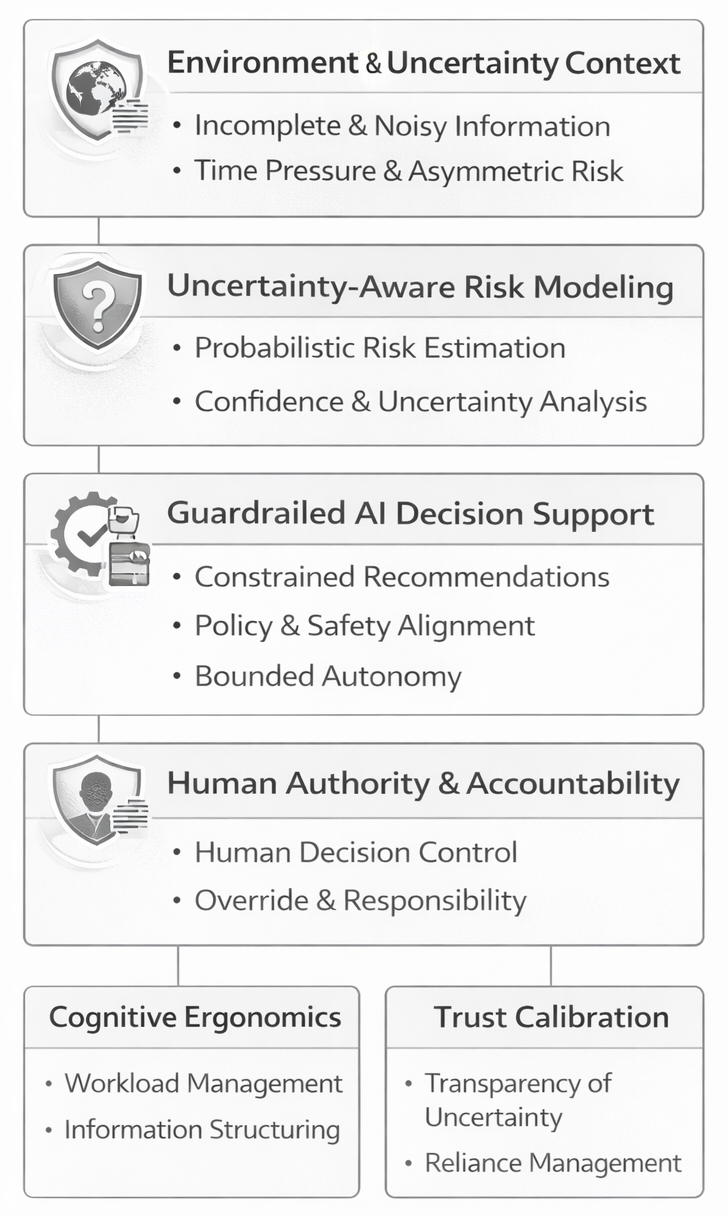
\includegraphics[width=0.60\linewidth]{fig_achdf_concept.png}
%DIFDELCMD <         \caption{Conceptual design layers of the Action-Centered Human--AI Decision Framework (ACHDF).
%DIFDELCMD < The framework structures human--AI decision support into four layered components: environment and uncertainty context, uncertainty-aware risk modeling, guardrailed AI decision support, and preserved human authority and accountability. Trust calibration and cognitive ergonomics operate as cross-cutting design considerations that influence interaction quality and reliable action execution under uncertainty.}
%DIFDELCMD <         \label{fig:achdf_concept}
%DIFDELCMD <     \end{figure}
%DIFDELCMD < %%%
\DIFdelend \DIFaddbegin \begin{figure}[t]
        \centering
        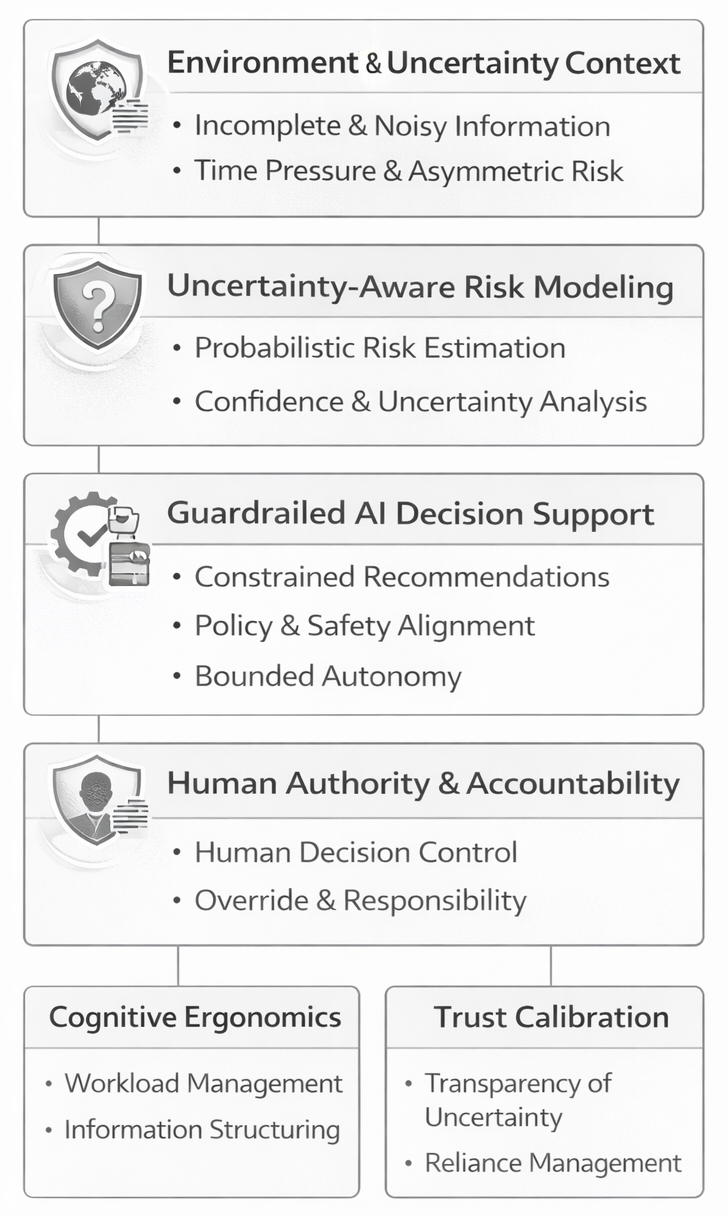
\includegraphics[width=0.60\linewidth]{fig_achdf_concept.png}
        \caption{Conceptual design layers of the Action-Centered Human--AI Decision Framework (ACHDF).
The framework structures human--AI decision support into four layered components: environment and uncertainty context, uncertainty-aware risk modeling, guardrailed AI decision support, and preserved human authority and accountability. Trust and cognitive workload are design considerations that guided interface design and are measured as evaluation outcomes. They are not adapted at run time (Table~\ref{tab:constructs}).}
        \label{fig:achdf_concept}
    \end{figure}
\DIFaddend 

    \DIFdelbegin %DIFDELCMD < \begin{figure}[t]
%DIFDELCMD <         \centering
%DIFDELCMD <         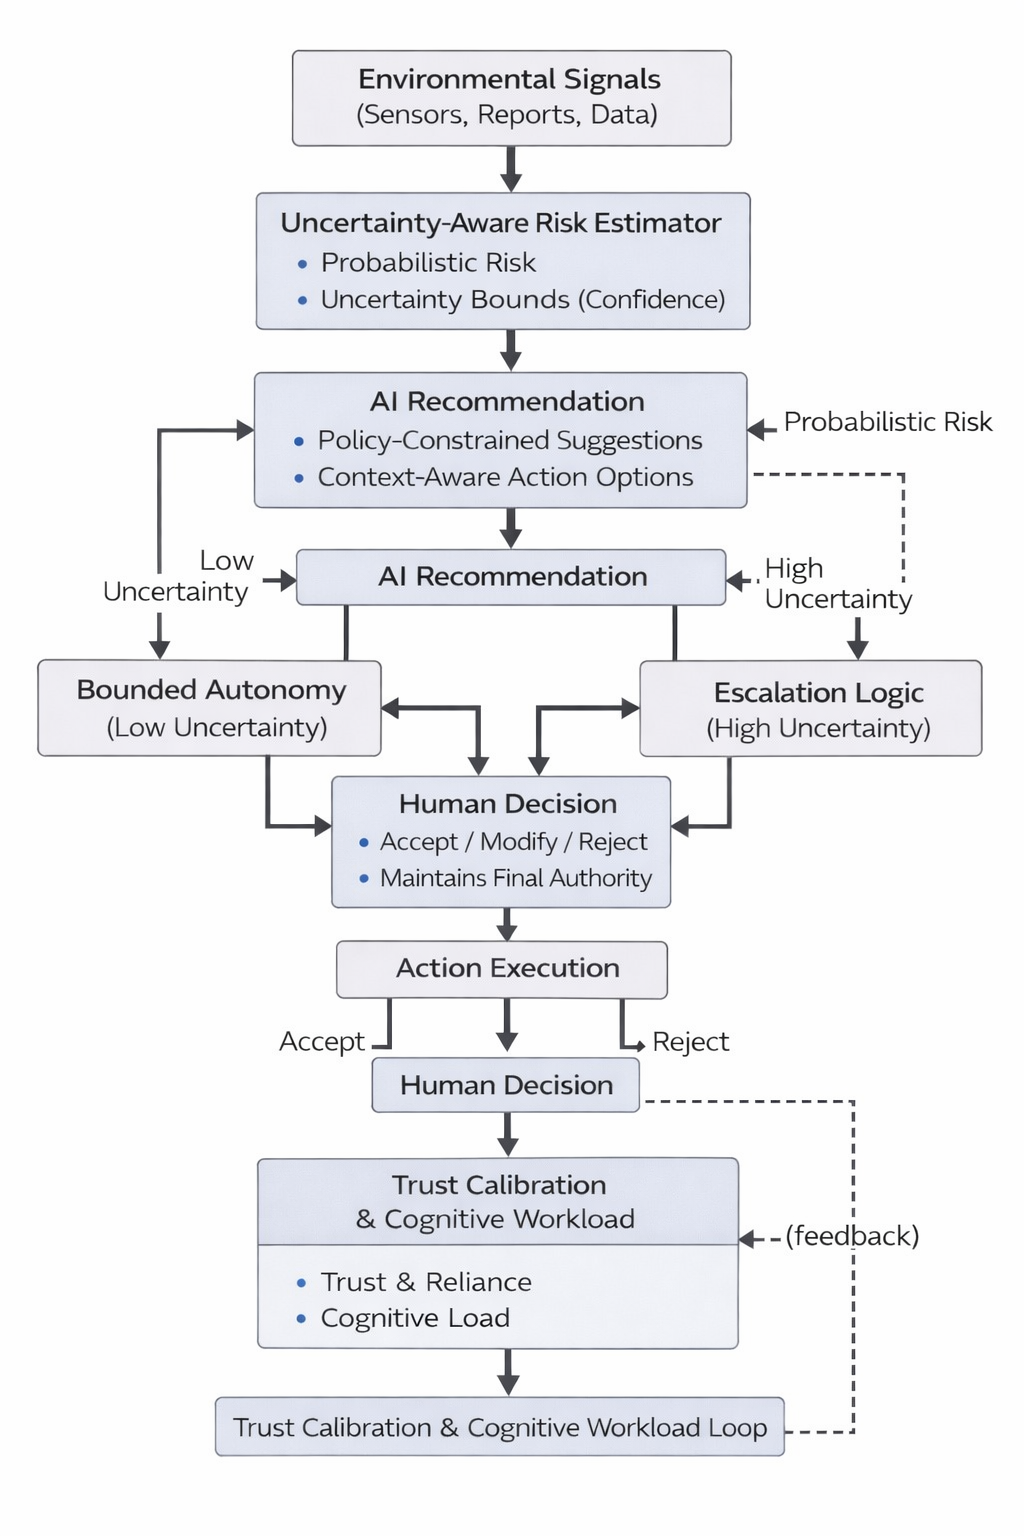
\includegraphics[width=0.95\linewidth]{fig_system_overview.png}
%DIFDELCMD <         \caption{Operational workflow of the proposed human--AI decision system.
%DIFDELCMD < Uncertainty-aware function allocation dynamically shifts decision authority between bounded autonomy and human-in-the-loop escalation.}
%DIFDELCMD <         \label{fig:system_overview}
%DIFDELCMD <     \end{figure}
%DIFDELCMD < %%%
\DIFdelend \DIFaddbegin \begin{figure}[t]
        \centering
        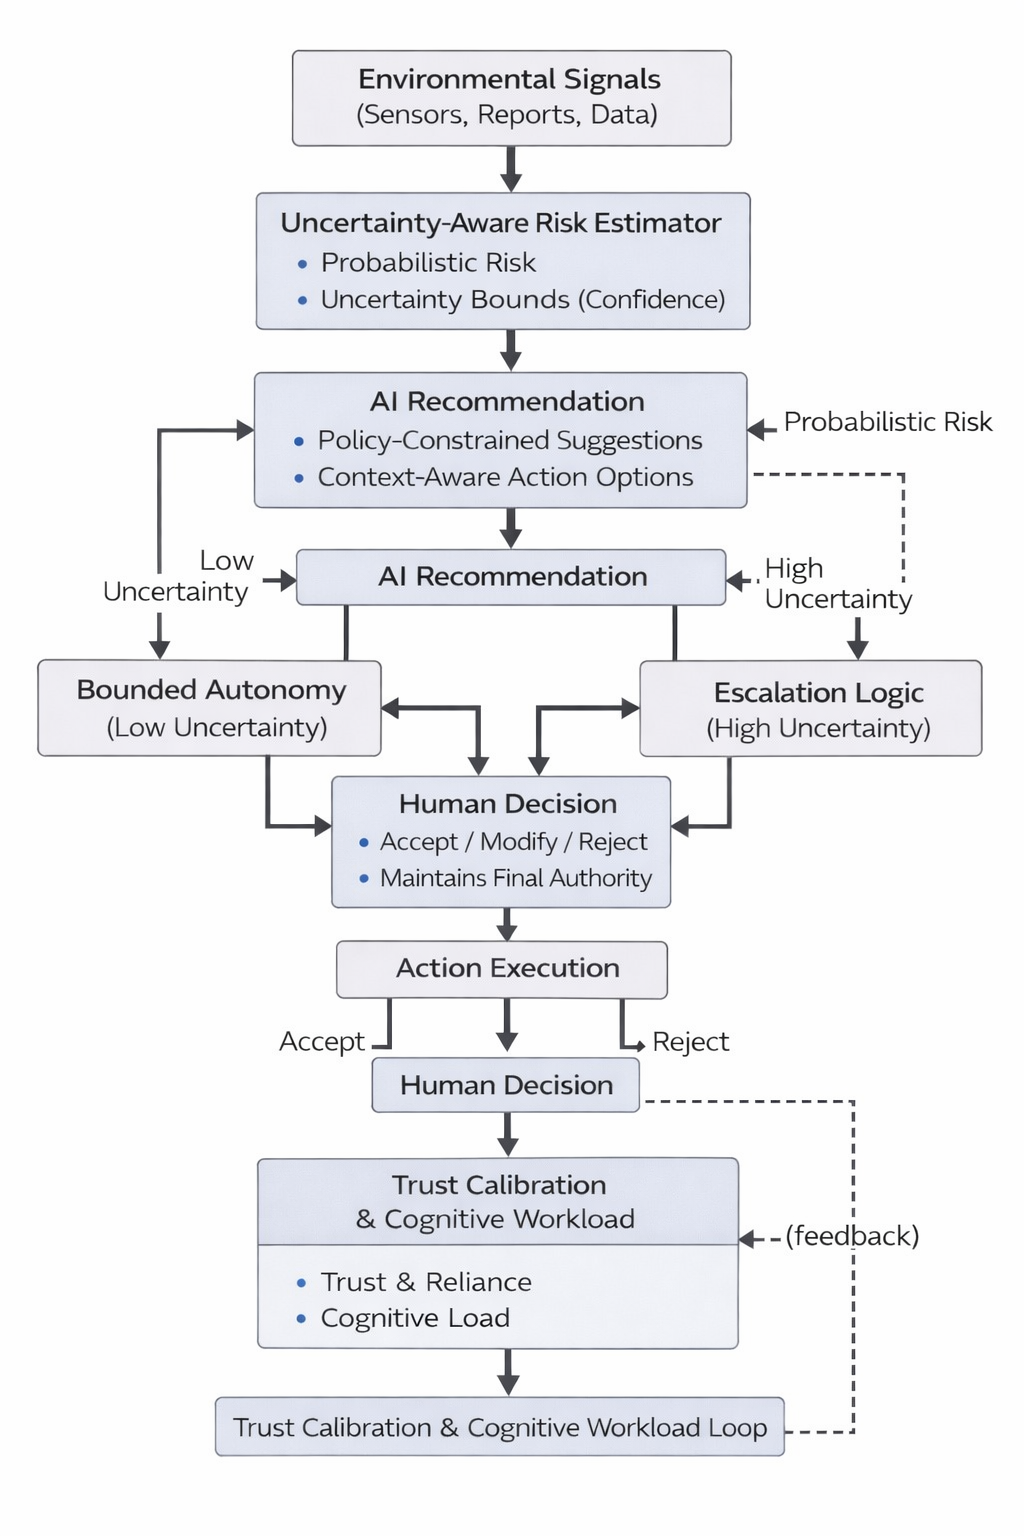
\includegraphics[width=0.95\linewidth]{fig_system_overview.png}
        \caption{Operational workflow of the proposed human--AI decision system.
Depending on estimated uncertainty, action criticality, and policy checks, the system either presents a bounded recommendation or escalates the case for human review with evidence and options. In both modes, the human operator holds final decision and execution authority.}
        \label{fig:system_overview}
    \end{figure}
\DIFaddend 

    \section{System Overview and Architecture}
    \DIFdelbegin \DIFdel{This section is intended to introduce }\DIFdelend \DIFaddbegin \label{sec:system}
    \DIFadd{This section introduces }\DIFaddend the proposed human--AI decision system \DIFdelbegin \DIFdel{. In addition, it is intended to introduce the architectural elementsof the proposed human--AI decision system. The proposed human--AI decision system is intended to be }\DIFdelend \DIFaddbegin \DIFadd{and its architectural elements. The system is }\DIFaddend non-autonomous and human-centric\DIFdelbegin \DIFdel{. It is intended to have a balanced approach to human and algorithmic decision-making. The architectural elements of the proposed human--AI decision system are based on }\DIFdelend \DIFaddbegin \DIFadd{: the AI analyzes information and proposes options, and the human decides and acts. The architecture follows }\DIFaddend the \textbf{Action-Centered Human--AI Decision Framework (ACHDF)}\DIFdelbegin \DIFdel{. In the proposed framework, there is a significant emphasis on human action execution as the primary goal of the system}\DIFdelend \DIFaddbegin \DIFadd{, which, following the joint cognitive systems perspective \cite{Hollnagel2005JCS,Woods2006JCS}, treats the human operator and the AI as one decision system and takes appropriate human action as the system's goal}\DIFaddend .

    A conceptual overview of the proposed action-centered architecture is illustrated in Fig.~\ref{fig:achdf_concept}.
As shown in the figure, ACHDF is organized into four primary design layers. The \emph{environment and uncertainty context} layer captures incomplete, time-pressured, and asymmetric risk conditions that characterize high-stakes decision ecologies. Built on top of this, the \emph{uncertainty-aware risk modeling} layer produces probabilistic risk estimates together with explicit confidence and uncertainty bounds. These estimates are then translated into constrained, policy-aligned options within the \emph{guardrailed AI decision support} layer, which ensures that generated recommendations remain consistent with operational and safety constraints. Finally, the \emph{human authority and accountability} layer preserves human control through oversight, override, and responsibility mechanisms. The two cross-cutting elements \DIFdelbegin \DIFdel{shown }\DIFdelend at the bottom of the figure\DIFdelbegin \DIFdel{—trust calibration }\DIFdelend \DIFaddbegin \DIFadd{, trust }\DIFaddend and cognitive ergonomics\DIFdelbegin \DIFdel{—continuously shape how information is presented so that operators can act reliably under uncertainty}\DIFdelend \DIFaddbegin \DIFadd{, are design considerations. They determined which cues are shown (e.g., explicit uncertainty indicators) and how much information is shown at once. The implemented system does not measure them or adapt to them at run time}\DIFaddend .

The \DIFdelbegin \DIFdel{dynamic operationalization }\DIFdelend \DIFaddbegin \DIFadd{run-time behavior }\DIFaddend of these layers \DIFdelbegin \DIFdel{in real-time decision making }\DIFdelend is depicted in Fig.~\ref{fig:system_overview}.
\DIFdelbegin \DIFdel{This workflow view emphasizes how uncertainty-aware function allocation governs the interaction loop between AI and the human operator. When model confidence is high and risk is bounded}\DIFdelend \DIFaddbegin \DIFadd{When model uncertainty is low and the action is not critical}\DIFaddend , the system \DIFdelbegin \DIFdel{can provide }\DIFdelend \DIFaddbegin \DIFadd{presents a }\DIFaddend tightly scoped, action-oriented \DIFdelbegin \DIFdel{recommendations under bounded autonomy. As uncertaintyor potential impact increases, the escalation logic routes decisions to a human-in-the-loop review process, where }\DIFdelend \DIFaddbegin \DIFadd{recommendation. We call this mode \emph{bounded autonomy}. The term refers only to the AI's freedom in \emph{generating} a recommendation, which is bounded by guardrails. It does not mean that the AI executes actions or holds decision authority. When uncertainty, criticality, or a policy check exceeds its threshold, the system switches to \emph{escalation}: instead of a single recommendation, it presents the evidence and the available options and explicitly asks the operator to review them, and }\DIFaddend the operator can approve, modify, or reject the suggested action. \DIFdelbegin \DIFdel{The feedback paths shown in the figure highlight how action outcomes and operator responses contribute to ongoing trust calibration and workload management, forming a closed human--AI decision loop oriented toward reliable action execution rather than mere prediction display}\DIFdelend \DIFaddbegin \DIFadd{Thus, what varies between the two modes is the \emph{level and form of AI support}. Final decision and execution authority stays with the human in both modes. Operator responses and outcomes are logged for audit and for offline recalibration of the thresholds.
}

    \subsection{\DIFadd{Constructs and Their Roles}}
    \label{sec:constructs}
    \DIFadd{Table~\ref{tab:constructs} summarizes the role of each ACHDF construct, i.e., whether it is a design input, a system state, a design consideration, or an evaluation outcome, together with its operational definition in the implemented system}\DIFaddend .

\DIFaddbegin \begin{table*}[t]
\centering
\caption{ACHDF Constructs: Role, Operational Definition, and Implementation}
\label{tab:constructs}
\begin{tabular}{p{2.4cm} p{3.4cm} p{10.6cm}}
\toprule
\textbf{Construct} & \textbf{Role in ACHDF} & \textbf{Operational definition / implementation} \\
\midrule
Uncertainty $u$ & Design input; determines system mode & Dispersion of the posterior risk estimate (Section~\ref{sec:risk}); compared with threshold $\tau_u$. \\
Criticality $c$ & Design input; determines system mode & Severity of the consequences if the recommended action is wrong or delayed (cost of error); compared with threshold $\tau_c$. \\
Guardrails & Constraint on recommendation generation & Rule-based checks applied to every generated recommendation (Section~\ref{sec:guardrails}). A recommendation that fails a check is withheld and the case is escalated ($v=1$ in Algorithm~\ref{alg:escalation}). \\
Bounded autonomy & System mode (``recommend'') & The AI presents one scoped, guardrail-checked recommendation. The AI never executes actions; the human decides and acts. \\
Escalation & System mode (``escalate'') & Triggered if $u \ge \tau_u$, $c \ge \tau_c$, or a policy check fails ($v=1$). The system presents evidence and options and asks the operator to approve, modify, or reject. \\
Trust & Design consideration; secondary outcome & Shaped interface design (explicit uncertainty and criticality cues). Measured post-condition by questionnaire (Section~\ref{sec:measures}). Not adapted at run time. \\
Workload & Design consideration; secondary outcome & Shaped interface design (single consolidated view, action-oriented phrasing). Measured post-condition by NASA--TLX \cite{Hart1988}. Not adapted at run time. \\
Action execution & Primary outcome & Measured by AER (Section~\ref{sec:measures}). \\
\bottomrule
\end{tabular}
\end{table*}

    \DIFaddend \subsection{Design Goals and Human-in-the-Loop Principles}
    The design of the proposed system is informed by three key goals that are derived from the fundamental principles of ACHDF.

    \textbf{Goal 1 \DIFdelbegin \DIFdel{— }\DIFdelend \DIFaddbegin \DIFadd{--- }\DIFaddend Enabling Human Action Execution.}
    The \DIFdelbegin \DIFdel{proposed system must be able to }\DIFdelend \DIFaddbegin \DIFadd{system should }\DIFaddend support \emph{human action execution} effectively, as opposed to \DIFdelbegin \DIFdel{simply }\DIFdelend \DIFaddbegin \DIFadd{only }\DIFaddend improving situational awareness and prediction accuracy.
\DIFdelbegin \DIFdel{The key goal of the proposed system is therefore to enable effective human decision-making and action in operational settings.
}\DIFdelend 

    \textbf{Goal 2 \DIFdelbegin \DIFdel{— }\DIFdelend \DIFaddbegin \DIFadd{--- }\DIFaddend Supporting \DIFdelbegin \DIFdel{Calibrated }\DIFdelend \DIFaddbegin \DIFadd{Appropriate }\DIFaddend Trust.}
    The \DIFdelbegin \DIFdel{proposed system must }\DIFdelend \DIFaddbegin \DIFadd{system should }\DIFaddend support appropriate trust \DIFdelbegin \DIFdel{calibration }\DIFdelend \DIFaddbegin \DIFadd{\cite{Lee2004} }\DIFaddend by making its uncertainty, model limitations, and potential failure modes explicit\DIFdelbegin \DIFdel{. By doing so, the proposed system enables users to develop a realistic understanding of when to trust the system's }\DIFdelend \DIFaddbegin \DIFadd{, so that users can judge when to rely on its }\DIFaddend outputs and when to \DIFdelbegin \DIFdel{trust human }\DIFdelend \DIFaddbegin \DIFadd{rely on their own }\DIFaddend judgment.

    \textbf{Goal 3 \DIFdelbegin \DIFdel{- }\DIFdelend \DIFaddbegin \DIFadd{--- }\DIFaddend Preserving Human Authority.}
    The system \DIFdelbegin \DIFdel{shall ensure the preservation of }\DIFdelend \DIFaddbegin \DIFadd{should preserve }\DIFaddend human authority in high-risk decisions\DIFdelbegin \DIFdel{by incorporating human-in-the-loop mechanisms and bounded autonomy. This means that, in safety-critical or ethically critical situations, the system will ensure that human operators have }\DIFdelend \DIFaddbegin \DIFadd{. Human operators always hold }\DIFaddend the final decision-making \DIFdelbegin \DIFdel{authority, avoiding over-reliance on automation or artificial intelligence}\DIFdelend \DIFaddbegin \DIFadd{and execution authority}\DIFaddend .

    To \DIFdelbegin \DIFdel{ensure that these goalsare achieved, the system will employ a human--AI collaboration paradigm, where the AI will be used to provide }\DIFdelend \DIFaddbegin \DIFadd{meet these goals, the AI provides }\DIFaddend decision scaffolding and action-oriented recommendations, and the human \DIFdelbegin \DIFdel{will have the final responsibility }\DIFdelend \DIFaddbegin \DIFadd{remains responsible }\DIFaddend for executing actions. \DIFdelbegin \DIFdel{The system will employ automation that assists in information synthesis and option generation, but will not be used for executing irreversible actions. This ensures the implementationof the concept of }\DIFdelend \DIFaddbegin \DIFadd{In the terms of Parasuraman \emph{et al.} \cite{Parasuraman2000LOA}, the system automates information analysis and decision selection, but not action implementation. The level and form of support are adapted to the estimated uncertainty and the criticality of the action (}\DIFaddend uncertainty-governed \DIFdelbegin \DIFdel{function allocation, where the level of automation will be dynamically adapted according to the level of uncertainty and criticality of actions}\DIFdelend \DIFaddbegin \DIFadd{adaptation of support)}\DIFaddend .

    \subsection{Probabilistic Risk Estimation With Uncertainty}
    \DIFdelbegin \DIFdel{The heart of the system is a probabilistic }\DIFdelend \DIFaddbegin \label{sec:risk}
    \DIFadd{The }\DIFaddend risk estimation module \DIFdelbegin \DIFdel{that provides calibrated risk assessments along }\DIFdelend \DIFaddbegin \DIFadd{provides risk assessments together }\DIFaddend with uncertainty representations. \DIFdelbegin \DIFdel{Unlike many models that produce point estimateresults, the model provides posterior risk distributions that include data-driven variability and epistemic uncertainty .
}\DIFdelend \DIFaddbegin \DIFadd{Rather than a point estimate, the module outputs a posterior risk distribution, from which the risk level $r$ and the uncertainty $u$ are derived.
    This paper focuses on how the risk estimate and its uncertainty are used in the human--AI interaction, not on the risk model itself. The model's estimation procedure and calibration are therefore not evaluated here (Section~\ref{sec:lim_reporting}).
}\DIFaddend 

    \DIFdelbegin \DIFdel{\textbf{Role 1 in ACHDF.}
    These estimates of uncertainty are a crucial part of the decision logic.
}\DIFdelend \DIFaddbegin \DIFadd{\textbf{Role in ACHDF.}
    }\DIFaddend The risk level is interpreted \DIFdelbegin \DIFdel{in conjunction with the confidence intervals to determine }\DIFdelend \DIFaddbegin \DIFadd{together with its uncertainty to decide }\DIFaddend whether the system \DIFdelbegin \DIFdel{should make recommendations on its own or whether the process should be deferred to humans. The system’s explicit representation of its own uncertainties helps to prevent the propagation of false precisionand supports the reasoning of the risk level in a way that mirrors the human decision-making process}\DIFdelend \DIFaddbegin \DIFadd{presents a bounded recommendation or escalates (Algorithm~\ref{alg:escalation}). Explicitly representing uncertainty is intended to avoid conveying false precision}\DIFaddend .

    \subsection{Guardrailed AI Recommendation Module}
    \DIFdelbegin \DIFdel{To make risk estimates actionable and provide appropriate recommendations, a }\DIFdelend \DIFaddbegin \label{sec:guardrails}
    \DIFadd{A }\DIFaddend generative AI module \DIFdelbegin \DIFdel{is used by the system.
}\DIFdelend \DIFaddbegin \DIFadd{converts the risk estimate into a recommended action and a short justification.
}\DIFaddend 

    \DIFdelbegin \DIFdel{\textbf{Role 2 in ACHDF}
    The system is constrained by a number of layers of structural guardrails that provide assurance with regard to reliability, consistency, and compliance with policies.
These guardrails ensure that the recommendations generated by the system align with the risk estimates that were made previously and that there is no contradiction with those estimates.There are also further constraints that restrict the scope of recommendations based on }\DIFdelend \DIFaddbegin \DIFadd{\textbf{Role in ACHDF.}
    Every generated recommendation passes through guardrails before it is shown: (i) a \emph{consistency check} ensures that the recommended action does not contradict the risk estimate (e.g., no ``no action needed'' message when $r \ge \tau_r$); (ii) a \emph{scope check} ensures that the recommendation is selected from the set of permitted actions for the scenario; and (iii) a \emph{policy check} ensures compliance with }\DIFaddend operational and safety \DIFdelbegin \DIFdel{considerations. These recommendations also provide context cues that indicate the criticality and confidence levels associated with them, thereby avoiding information processing and facilitating a smooth transition to decisions and actions under pressure}\DIFdelend \DIFaddbegin \DIFadd{rules. A recommendation that fails any check is not shown; instead, the case is escalated ($v=1$).
    The specific rule sets, the generative model configuration, and the scale and thresholds for criticality are not reported in this paper (Section~\ref{sec:lim_reporting}).
    Each recommendation is displayed with its criticality and confidence cues}\DIFaddend . By bounding the generative \DIFdelbegin \DIFdel{results }\DIFdelend \DIFaddbegin \DIFadd{output }\DIFaddend within a structured decision process, the \DIFdelbegin \DIFdel{system harnesses the flexibility of generative AI while also limiting the risks of hallucination and overgeneralization, thereby ensuring that AI support is }\DIFdelend \DIFaddbegin \DIFadd{module aims to keep AI support }\DIFaddend assistive rather than prescriptive \DIFdelbegin \DIFdel{.
    }%DIFDELCMD < \begin{algorithm}[t]
%DIFDELCMD <         \caption{Uncertainty-aware escalation and human override policy}
%DIFDELCMD <         \label{alg:escalation}
%DIFDELCMD <         \begin{algorithmic}[1]
%DIFDELCMD <             \Require risk estimate $r$, uncertainty $u$, action criticality $c$
%DIFDELCMD <             \Require thresholds $\tau_r, \tau_u, \tau_c$
%DIFDELCMD <             \State $\textsc{mode} \leftarrow \text{``assist''}$
%DIFDELCMD <             \If{$u \ge \tau_u$ \textbf{or} $c \ge \tau_c$}
%DIFDELCMD <             \State $\textsc{mode} \leftarrow \text{``escalate''}$ \Comment{route to human review}
%DIFDELCMD <             \ElsIf{$r \ge \tau_r$}
%DIFDELCMD <             \State $\textsc{mode} \leftarrow \text{``recommend''}$
%DIFDELCMD <             \Else
%DIFDELCMD <             \State $\textsc{mode} \leftarrow \text{``monitor''}$
%DIFDELCMD <             \EndIf
%DIFDELCMD <             \If{$\textsc{mode} = \text{``escalate''}$}
%DIFDELCMD <             \State Present evidence and options to operator
%DIFDELCMD <             \State Operator selects: approve / modify / reject
%DIFDELCMD <             \Else
%DIFDELCMD <             \State Generate bounded recommendation via guardrails
%DIFDELCMD <             \EndIf
%DIFDELCMD <             \State Log decision context and outcome for audit and calibration
%DIFDELCMD <         \end{algorithmic}
%DIFDELCMD <     \end{algorithm}
%DIFDELCMD <     %%%
\DIFdelend \DIFaddbegin \DIFadd{and to limit hallucination and overgeneralization.
    }\begin{algorithm}[t]
        \caption{Uncertainty-aware escalation and human override policy}
        \label{alg:escalation}
        \begin{algorithmic}[1]
            \Require risk estimate $r$, uncertainty $u$, action criticality $c$
            \Require policy-violation flag $v \in \{0,1\}$ from guardrail checks
            \Require thresholds $\tau_r, \tau_u, \tau_c$
            \State $\textsc{mode} \leftarrow \text{``assist''}$
            \If{$u \ge \tau_u$ \textbf{or} $c \ge \tau_c$ \textbf{or} $v = 1$}
            \State $\textsc{mode} \leftarrow \text{``escalate''}$ \Comment{route to human review}
            \ElsIf{$r \ge \tau_r$}
            \State $\textsc{mode} \leftarrow \text{``recommend''}$ \Comment{bounded autonomy}
            \Else
            \State $\textsc{mode} \leftarrow \text{``monitor''}$
            \EndIf
            \If{$\textsc{mode} = \text{``escalate''}$}
            \State Present evidence and options to operator
            \State Operator selects: approve / modify / reject
            \ElsIf{$\textsc{mode} = \text{``recommend''}$}
            \State Present guardrail-checked recommendation
            \State Operator decides and executes (or overrides)
            \EndIf
            \State Log decision context and outcome for audit and calibration
        \end{algorithmic}
    \end{algorithm}
\DIFaddend 

\subsection{Human Override and Escalation Mechanisms}
\DIFdelbegin \DIFdel{The escalation process, as described }\DIFdelend \DIFaddbegin \DIFadd{Escalation follows the policy }\DIFaddend in Algorithm~\ref{alg:escalation}\DIFdelbegin \DIFdel{, is linked to an uncertainty-aware policy that is used to dynamically allocate authority depending on the level of uncertainty and the criticality of the actions taken. The human override and escalation mechanism is an important part of the overall system architecture.
The system automatically escalates decisions to human operators if the level of uncertainty is above certain thresholds, the potential impact of the recommendation is high, and if certain policy constraints are violated. In fact, escalation }\DIFdelend \DIFaddbegin \DIFadd{. The system escalates a case to the operator if \emph{any} of three conditions holds: the uncertainty exceeds $\tau_u$, the criticality of the action exceeds $\tau_c$, or a guardrail policy check fails ($v=1$). Escalation }\DIFaddend is not a failure mode\DIFdelbegin \DIFdel{but a decision to escalate to ensure accountability under uncertain conditions.
The operators are free to either }\DIFdelend \DIFaddbegin \DIFadd{. It is a deliberate change in the form of support that keeps the operator accountable under uncertainty.
In every mode, operators can }\DIFaddend accept, modify, or reject the \DIFdelbegin \DIFdel{decision recommended by the AIsystem}\DIFdelend \DIFaddbegin \DIFadd{AI's recommendation}\DIFaddend , and all of these operations are \DIFdelbegin \DIFdel{recorded for accountabilitypurposes. This minimization of processing of superfluous information is also beneficial for the management of cognitive workload for }\DIFdelend \DIFaddbegin \DIFadd{logged for accountability. Showing a single consolidated recommendation in routine cases is intended to reduce the amount of information operators must process in }\DIFaddend time-critical situations.
This \DIFdelbegin \DIFdel{dynamic allocation of autonomy allows the system to offer effective assistance in regular situationsand, at the same time, allow human control }\DIFdelend \DIFaddbegin \DIFadd{adaptation of the level of support (a scoped recommendation in routine situations, a full review }\DIFaddend in uncertain or \DIFdelbegin \DIFdel{risky situations, thus striking a proper balance between performance and safety, as per the existing design principles for human--machine systems, which provides a platform for the ACHDF design principles proposed later in the paper}\DIFdelend \DIFaddbegin \DIFadd{critical ones) follows established principles of adaptive automation \cite{Parasuraman2000LOA,Scerbo2007} and does not transfer decision authority to the AI}\DIFaddend .

\DIFdelbegin %DIFDELCMD < \begin{table*}[t]
%DIFDELCMD < \centering
%DIFDELCMD < \caption{Transferability of ACHDF Design Principles Across Decision Ecologies}
%DIFDELCMD < \label{tab:achdf_transferability}
%DIFDELCMD < \begin{tabular}{p{3cm} p{3.2cm} p{3.2cm} p{2.8cm} p{3.9cm}}
%DIFDELCMD < \hline
%DIFDELCMD < \textbf{Decision Domain} &
%DIFDELCMD < \textbf{Primary Sources of Uncertainty} &
%DIFDELCMD < \textbf{Asymmetry of Error Costs} &
%DIFDELCMD < \textbf{Time Pressure Characteristics} &
%DIFDELCMD < \textbf{Role of Uncertainty-Aware Function Allocation} \\
%DIFDELCMD < \hline
%DIFDELCMD < Disaster Response &
%DIFDELCMD < Incomplete situational awareness, noisy sensor and report data, rapidly evolving conditions &
%DIFDELCMD < Delayed action leads to loss of life or property; false alarms incur operational cost &
%DIFDELCMD < Severe time pressure with dynamic escalation requirements &
%DIFDELCMD < AI provides bounded, action-oriented recommendations under low uncertainty; high uncertainty triggers human-in-the-loop escalation to preserve accountability \\
%DIFDELCMD < 

%DIFDELCMD < Autonomous Driving Supervision &
%DIFDELCMD < Perception uncertainty, rare edge cases, environment variability &
%DIFDELCMD < False negatives may cause accidents; false positives reduce efficiency and trust &
%DIFDELCMD < Sub-second to seconds-level response requirements &
%DIFDELCMD < Low-uncertainty situations allow bounded autonomy; ambiguous or novel situations escalate to human supervision and override \\
%DIFDELCMD < 

%DIFDELCMD < Medical AI (Triage / Diagnosis) &
%DIFDELCMD < Incomplete patient data, population-to-individual generalization limits &
%DIFDELCMD < False negatives risk patient harm; false positives cause overtreatment &
%DIFDELCMD < Moderate to high time pressure depending on clinical context &
%DIFDELCMD < AI assists with risk stratification and option generation; high uncertainty or high criticality decisions defer to clinicians \\
%DIFDELCMD < 

%DIFDELCMD < Military Safety Automation &
%DIFDELCMD < Adversarial uncertainty, incomplete intelligence, strategic deception &
%DIFDELCMD < Incorrect action may cause catastrophic or irreversible consequences &
%DIFDELCMD < High time pressure combined with strategic deliberation &
%DIFDELCMD < AI supports sensemaking and constrained recommendations; final decision authority remains with human operators under uncertainty \\
%DIFDELCMD < 

%DIFDELCMD < \hline
%DIFDELCMD < \end{tabular}
%DIFDELCMD < \end{table*}
%DIFDELCMD < %%%
\DIFdelend \DIFaddbegin \begin{table*}[t]
\centering
\caption{Hypothesized Mapping of ACHDF Design Principles to Other Decision Ecologies (Not Empirically Tested)}
\label{tab:achdf_transferability}
\begin{tabular}{p{3cm} p{3.2cm} p{3.2cm} p{2.8cm} p{3.9cm}}
\hline
\textbf{Decision Domain} &
\textbf{Primary Sources of Uncertainty} &
\textbf{Asymmetry of Error Costs} &
\textbf{Time Pressure Characteristics} &
\textbf{Potential Role of Uncertainty-Aware Support Adaptation} \\
\hline
Disaster Response (evaluated here) &
Incomplete situational awareness, noisy sensor and report data, rapidly evolving conditions &
Delayed action leads to loss of life or property; false alarms incur operational cost &
Severe time pressure with dynamic escalation requirements &
AI provides bounded, action-oriented recommendations under low uncertainty; high uncertainty triggers human-in-the-loop escalation to preserve accountability \\

Autonomous Driving Supervision &
Perception uncertainty, rare edge cases, environment variability &
False negatives may cause accidents; false positives reduce efficiency and trust &
Sub-second to seconds-level response requirements &
Low-uncertainty situations allow bounded recommendations; ambiguous or novel situations escalate to human supervision and override \\

Medical AI (Triage / Diagnosis) &
Incomplete patient data, population-to-individual generalization limits &
False negatives risk patient harm; false positives cause overtreatment &
Moderate to high time pressure depending on clinical context &
AI assists with risk stratification and option generation; high uncertainty or high criticality decisions defer to clinicians \\

Military Safety Automation &
Adversarial uncertainty, incomplete intelligence, strategic deception &
Incorrect action may cause catastrophic or irreversible consequences &
High time pressure combined with strategic deliberation &
AI supports sensemaking and constrained recommendations; final decision authority remains with human operators under uncertainty \\

\hline
\end{tabular}
\end{table*}
\DIFaddend 


\subsection{\DIFdelbegin \DIFdel{ACHDF }\DIFdelend \DIFaddbegin \DIFadd{Potential }\DIFaddend Transferability Across Decision Ecologies}
\DIFdelbegin \DIFdel{Although the system architecture is instantiated and verified in the context of disaster response, the design principlesare not domain-specific in nature. On the contrary, the architecture presented here is more aligned with a general }\DIFdelend \DIFaddbegin \DIFadd{The architecture was instantiated and evaluated only in disaster response. The design principles, however, address a structural }\DIFaddend class of \emph{decision ecologies} \DIFdelbegin \DIFdel{that are }\DIFdelend characterized by high uncertainty, \DIFdelbegin \DIFdel{asymmetrical costs of errors, timing pressures}\DIFdelend \DIFaddbegin \DIFadd{asymmetric costs of error, time pressure}\DIFaddend , and human accountability. \DIFdelbegin \DIFdel{The \textbf{Action-Centered Human--AI Decision Framework (ACHDF)} is intended to be more general in nature to cover a range of different safety-critical domains that have similar structural characteristics.
}%DIFDELCMD < 

%DIFDELCMD < %%%
\DIFdel{In order to further illustrate the general nature of the design principles presented in this work, Table\ref{tab:achdf_transferability} provides a decision ecology mapping that illustrates the transferability of the design principles to different application domains that are presented in this paper, such as the supervision of autonomous driving , medical AI in the context of medical }\DIFdelend \DIFaddbegin \DIFadd{Table~\ref{tab:achdf_transferability} maps these characteristics to three other domains (autonomous driving supervision, medical }\DIFaddend triage or diagnostic support\DIFdelbegin \DIFdel{systems, or }\DIFdelend \DIFaddbegin \DIFadd{, and }\DIFaddend military safety automation\DIFdelbegin \DIFdel{systems. Despite the varying nature of the uncertainty in each of the application domains considered in this paper, the role of }\DIFdelend \DIFaddbegin \DIFadd{) to show where }\DIFaddend uncertainty-aware \DIFdelbegin \DIFdel{function allocation is similar in nature. The contribution of this work is not about optimizing any particulardomain or application scenario in the context of human--AI decisions under uncertainty}\DIFdelend \DIFaddbegin \DIFadd{adaptation of support \emph{could} play a similar role. This mapping is a hypothesis for future work, not an empirical result. In particular, time scales, operator expertise, and regulatory constraints differ substantially across these domains (Section~\ref{sec:limitations})}\DIFaddend .

    % -------------------------------\input{./060-evaluation}
    \section{Experimental Design and Methods}

    \DIFdelbegin \DIFdel{In this section , we describe the design of the experiments that can be used to test the proposed human--AI decision system . In our case, we aimed to isolate the effect of AI support on human action execution, response behavior, and subjective experience. In general, our design of experiments follows the usual practice of designing experiments to evaluate human--machine systems, where experiments are defined with clear conditions for baseline and treatment cases}\DIFdelend \DIFaddbegin \DIFadd{This section describes the controlled user study that compared the ACHDF-based system with a conventional dashboard. The study is the only empirical evaluation reported in this paper. Details that could not be reported because the underlying materials or trial-level data were not available are listed in Section~\ref{sec:lim_reporting}}\DIFaddend .

    \subsection{Study Design and Conditions\DIFdelbegin \DIFdel{(Baseline vs.\ AI-Assisted)}\DIFdelend }

    \DIFdelbegin \DIFdel{A }\DIFdelend \DIFaddbegin \DIFadd{We used a }\DIFaddend within-subjects design \DIFdelbegin \DIFdel{was employed in the experiment. In this design, the participants are presented with the same decision-making task in two different }\DIFdelend \DIFaddbegin \DIFadd{with two }\DIFaddend conditions: a \emph{baseline} condition and an \emph{AI-assisted} \DIFdelbegin \DIFdel{condition. In the baseline condition, the participants were presented with the conventional dashboard-based interface. In the AI-assisted condition, the participants were presented with the proposed system that provides context-aware recommendations through the human--AI decision architecture.
    To avoid learning effects and order effects in the experiment, the presentation order of the two conditions is counterbalanced. The significance of the results is determined by conducting a paired test.In both the baseline and }\DIFdelend \DIFaddbegin \DIFadd{(ACHDF) condition. The order of the conditions was counterbalanced across participants to control for order and learning effects. Both conditions used the same underlying scenario data.
}

    \DIFadd{\textbf{Baseline condition.} Participants used a conventional dashboard that displayed the hazard and risk information for each scenario. The dashboard provided no AI-generated action recommendation, uncertainty indicator, criticality cue, or escalation prompt. Participants had to integrate the information themselves and decide on an action.
}

    \DIFadd{\textbf{AI-assisted condition.} Participants used the ACHDF-based interface, which displayed the same underlying information together with the ACHDF features described in Section~\ref{sec:system}: the risk estimate with an explicit uncertainty indicator, a criticality cue, and either a single guardrail-checked action recommendation (``recommend'' mode) or, when escalation was triggered, the evidence and options with a prompt to review them (``escalate'' mode). The decision logic is shown in Fig.~\ref{fig:system_overview} and Algorithm~\ref{alg:escalation}. Interface screenshots are not included (Section~\ref{sec:lim_reporting}).
}

    \DIFadd{Because the }\DIFaddend AI-assisted \DIFdelbegin \DIFdel{conditions, the same data is used. Hence, the difference in the performance between the two conditions is solely due to the presence of AI assistance}\DIFdelend \DIFaddbegin \DIFadd{condition differs from the baseline in several features at once (recommendation, action-oriented format, uncertainty cue, criticality cue, and escalation), the comparison estimates the effect of the integrated ACHDF configuration. It does not isolate the effect of any single feature}\DIFaddend .

    \subsection{Participants and \DIFdelbegin \DIFdel{Sampling Strategy}\DIFdelend \DIFaddbegin \DIFadd{Ethics}\DIFaddend }
    \DIFaddbegin \label{sec:participants}
\DIFaddend 

    \DIFdelbegin \DIFdel{The demographics of participants are presented in }\DIFdelend \DIFaddbegin \DIFadd{Fifty-two participants took part (}\DIFaddend Table~\ref{tab:participants}\DIFdelbegin \DIFdel{.
}%DIFDELCMD < 

%DIFDELCMD <     \begin{table}[t]
%DIFDELCMD < 

%DIFDELCMD <         \caption{Participant Demographics}
%DIFDELCMD < 

%DIFDELCMD <         \label{tab:participants}
%DIFDELCMD < 

%DIFDELCMD <         \centering
%DIFDELCMD < 

%DIFDELCMD <         \begin{tabular}{l c}
%DIFDELCMD < 

%DIFDELCMD <             \hline
%DIFDELCMD < 

%DIFDELCMD <             Characteristic & Value \\
%DIFDELCMD < 

%DIFDELCMD <             \hline
%DIFDELCMD < 

%DIFDELCMD <             Total participants & 52 \\
%DIFDELCMD < 

%DIFDELCMD <             Age range & 20--50s \\
%DIFDELCMD < 

%DIFDELCMD <             Gender & Mixed \\
%DIFDELCMD < 

%DIFDELCMD <             Technical background & Low--High \\
%DIFDELCMD < 

%DIFDELCMD <             Study design & Within-subjects \\
%DIFDELCMD < 

%DIFDELCMD <             \hline
%DIFDELCMD < 

%DIFDELCMD <         \end{tabular}
%DIFDELCMD < 

%DIFDELCMD <     \end{table}
%DIFDELCMD < 

%DIFDELCMD <     %%%
\DIFdel{The total number of participants recruited for the study was 52 in number. For the purpose of this study, participants }\DIFdelend \DIFaddbegin \DIFadd{). Participants }\DIFaddend were recruited using \DIFdelbegin \DIFdel{the stratified sampling technique in order to create diversity in terms of }\DIFdelend \DIFaddbegin \DIFadd{stratified sampling to obtain diversity in }\DIFaddend age, gender, and technical \DIFdelbegin \DIFdel{know-how. This technique has been selected due to the heterogeneity observed in operators in real-world }\DIFdelend \DIFaddbegin \DIFadd{background, reflecting the heterogeneity of operators in real }\DIFaddend decision environments. \DIFdelbegin %DIFDELCMD < 

%DIFDELCMD <     %%%
\DIFdel{All participants gave their informed consent prior to the experiment. Although participants }\DIFdelend \DIFaddbegin \DIFadd{Participants }\DIFaddend were not required to have prior \DIFdelbegin \DIFdel{knowledge in the domain area, training on the task interface was provided to all participants to create uniformity in terms of familiarity with the procedures}\DIFdelend \DIFaddbegin \DIFadd{domain expertise, and the sample was not composed specifically of trained emergency-management professionals (Section~\ref{sec:limitations}).
}

    \DIFadd{The study was not submitted to an institutional review board or ethics committee for review. It involved only a simulated decision task and post-task questionnaires and interviews, with no physical or medical intervention. Participation was voluntary, and all participants gave informed consent before the experiment.
}

    \DIFadd{\textbf{Sample size.} No a priori power analysis was reported for this study. A post hoc sensitivity analysis shows that, with $n=52$, a two-sided paired $t$-test at $\alpha=.05$ has 80\% power to detect a within-subject effect of $d_z \approx 0.40$ or larger. Effects smaller than this may not have been detected reliably}\DIFaddend .

    \DIFdelbegin \subsection{\DIFdel{Task Design and Procedure}}
%DIFAUXCMD
\addtocounter{subsection}{-1}%DIFAUXCMD
\DIFdelend \DIFaddbegin \begin{table}[t]
        \caption{Participant Demographics}
        \label{tab:participants}
        \centering
        \begin{tabular}{l c}
            \toprule
            Characteristic & Value \\
            \midrule
            Total participants & 52 \\
            Age range & 20s--50s \\
            Gender & Mixed \\
            Technical background & Low--high \\
            Domain expertise required & No \\
            Study design & Within-subjects \\
            \bottomrule
        \end{tabular}
    \end{table}
\DIFaddend 

    \DIFdelbegin \DIFdel{The participants were required to complete a set of time-sensitive }\DIFdelend \DIFaddbegin \subsection{\DIFadd{Decision Task and Procedure}}

    \DIFadd{Participants completed a series of time-limited }\DIFaddend decision tasks. \DIFdelbegin \DIFdel{These tasks involved understanding risk information and making a decision on whetheror not }\DIFdelend \DIFaddbegin \DIFadd{In each task, they interpreted risk information about an evolving hazard and decided whether, and how, }\DIFaddend to take a protective action. \DIFdelbegin \DIFdel{These decision tasks were aimed at capturing the essential aspects of a }\DIFdelend \DIFaddbegin \DIFadd{When the system escalated a case, participants could also defer the decision pending further confirmation. The tasks were designed to reproduce the essential characteristics of }\DIFaddend high-stakes \DIFdelbegin \DIFdel{decision situation. These aspects include changes in }\DIFdelend \DIFaddbegin \DIFadd{decisions: changing }\DIFaddend information, uncertainty, and \DIFdelbegin \DIFdel{unbalanced }\DIFdelend \DIFaddbegin \DIFadd{asymmetric }\DIFaddend error costs. \DIFdelbegin \DIFdel{The experiment involved a training period, and after that, the participants completed the task execution of both the experimental conditions. The participants were required }\DIFdelend \DIFaddbegin \DIFadd{Participants were instructed }\DIFaddend to focus on \DIFdelbegin \DIFdel{the efficacy of the }\DIFdelend \DIFaddbegin \DIFadd{taking the appropriate }\DIFaddend action rather than on \DIFdelbegin \DIFdel{the analysis of }\DIFdelend \DIFaddbegin \DIFadd{analyzing }\DIFaddend the information.
\DIFdelbegin \DIFdel{The system was used to record the decision processes and interaction of the participants. }%DIFDELCMD < 

%DIFDELCMD <     \begin{table}[t]
%DIFDELCMD <         \caption{Outcome measures used in the controlled study}
%DIFDELCMD <         \label{tab:measures}
%DIFDELCMD <         \centering
%DIFDELCMD <         \begin{tabular}{p{0.23\linewidth}p{0.70\linewidth}}
%DIFDELCMD <             \toprule
%DIFDELCMD <             \textbf{Measure} & \textbf{Operationalization} \\
%DIFDELCMD <             \midrule
%DIFDELCMD <             Response Latency & Time from presentation of actionable information to action execution. \\
%DIFDELCMD <             Cognitive Workload & NASA--TLX overall score and subscales (post-condition). \\
%DIFDELCMD <             Trust & Post-task Likert-type items on perceived reliability, predictability, and appropriateness of recommendations. \\
%DIFDELCMD <             Usability & Standard usability scale (post-condition). \\
%DIFDELCMD <             \bottomrule
%DIFDELCMD <         \end{tabular}
%DIFDELCMD <     \end{table}
%DIFDELCMD < 

%DIFDELCMD <     %%%
%DIF < ------------------------------------------------------
%DIFDELCMD < 

%DIFDELCMD <     \begin{figure}[t]
%DIFDELCMD <         \centering
%DIFDELCMD <         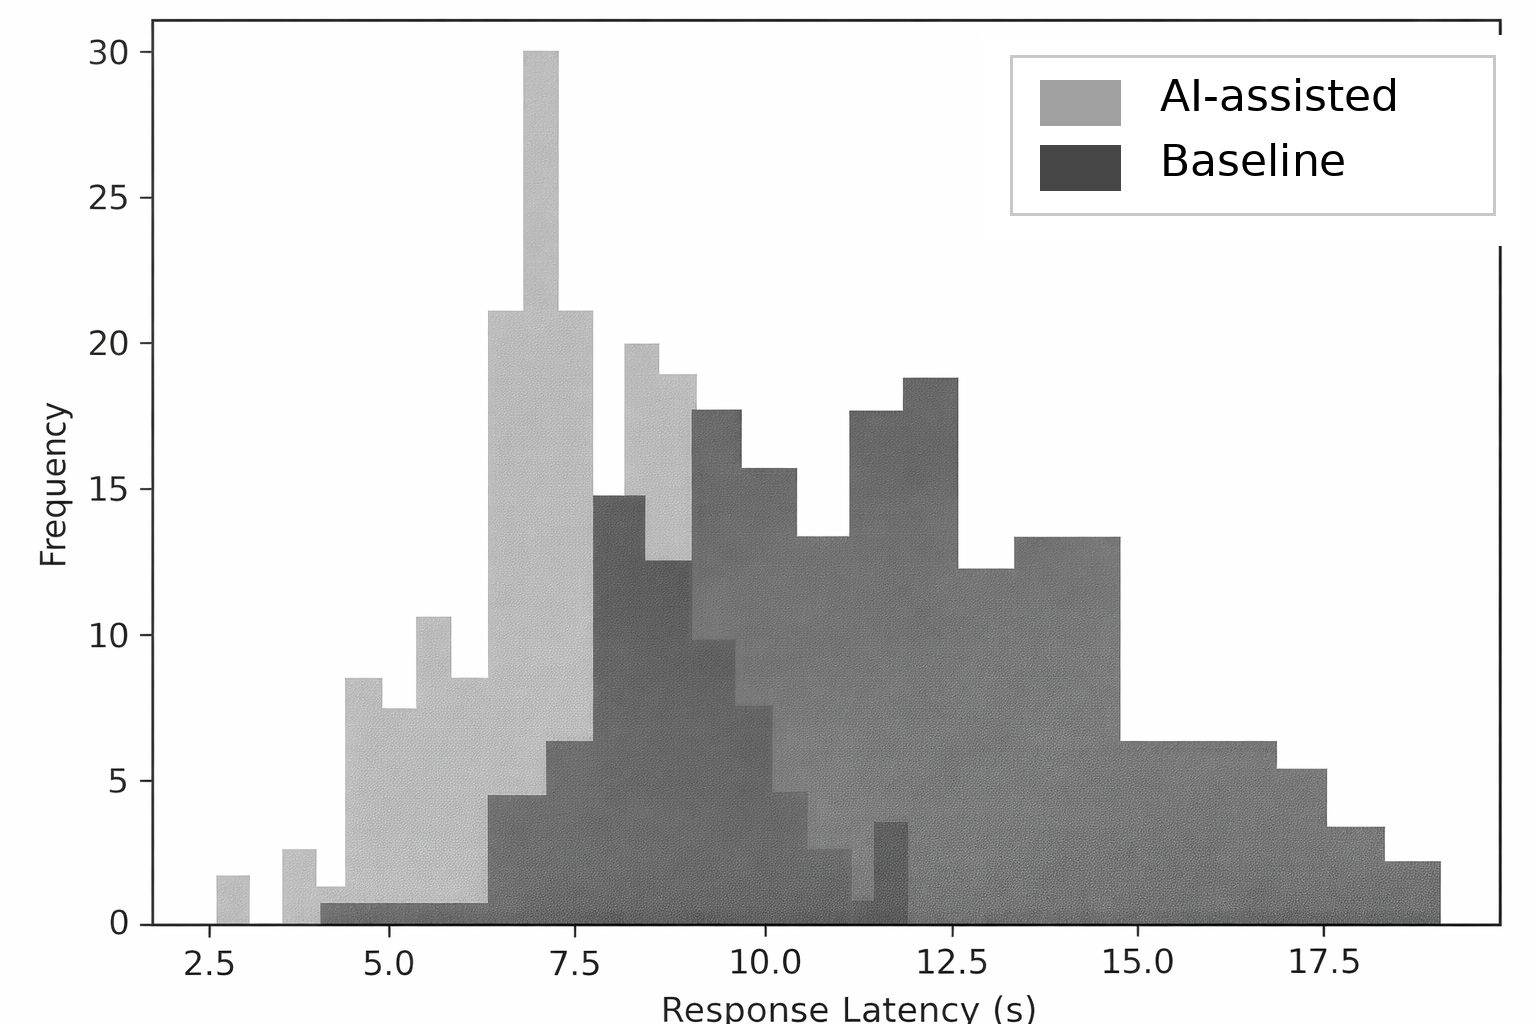
\includegraphics[width=0.9\linewidth]{fig_latency_distribution.png}
%DIFDELCMD <         \caption{Distribution of response latency under baseline and AI-assisted conditions. The distribution under the AI-assisted condition is left-shifted, indicating that the subjects made quicker transitions from risk interpretation to action execution.}
%DIFDELCMD <         \label{fig:latency_distribution}
%DIFDELCMD <     \end{figure}
%DIFDELCMD < 

%DIFDELCMD <     %%%
%DIF < ----------------------------------------------
    %DIFDELCMD < \begin{table}[t]
%DIFDELCMD <         \caption{Cognitive workload outcomes measured using NASA--TLX}
%DIFDELCMD <         \label{tab:workload}
%DIFDELCMD <         \centering
%DIFDELCMD <         \begin{tabular}{lcc}
%DIFDELCMD <             \toprule
%DIFDELCMD <             \textbf{NASA--TLX Dimension} & \textbf{Baseline} & \textbf{AI-assisted} \\
%DIFDELCMD <             \midrule
%DIFDELCMD <             Mental Demand & 63.4 (12.1) & 48.7 (10.5) \\
%DIFDELCMD <             Temporal Demand & 58.9 (11.4) & 44.2 (9.8) \\
%DIFDELCMD <             Effort & 61.7 (13.0) & 49.1 (11.2) \\
%DIFDELCMD <             Frustration & 55.3 (14.6) & 41.8 (12.3) \\
%DIFDELCMD <             \midrule
%DIFDELCMD <             Overall NASA--TLX & 59.8 (10.9) & 46.2 (9.6) \\
%DIFDELCMD <             \bottomrule
%DIFDELCMD <         \end{tabular}
%DIFDELCMD <     \end{table}
%DIFDELCMD < %%%
\DIFdelend 

    %DIF < ---------------------------------------------
    \DIFdelbegin %DIFDELCMD < \begin{table}[t]
%DIFDELCMD <         \caption{Trust and usability outcomes (post-task questionnaires)}
%DIFDELCMD <         \label{tab:trust_usability}
%DIFDELCMD <         \centering
%DIFDELCMD <         \begin{tabular}{lcc}
%DIFDELCMD <             \toprule
%DIFDELCMD <             \textbf{Measure} & \textbf{Baseline} & \textbf{AI-assisted} \\
%DIFDELCMD <             \midrule
%DIFDELCMD <             Perceived Reliability & 3.2 (0.7) & 4.1 (0.6) \\
%DIFDELCMD <             Perceived Appropriateness & 3.4 (0.6) & 4.3 (0.5) \\
%DIFDELCMD <             Predictability & 3.5 (0.8) & 4.2 (0.6) \\
%DIFDELCMD <             \midrule
%DIFDELCMD <             Overall Trust Score & 3.4 (0.6) & 4.2 (0.5) \\
%DIFDELCMD <             System Usability Score & 68.5 (11.2) & 81.7 (9.4) \\
%DIFDELCMD <             \bottomrule
%DIFDELCMD <         \end{tabular}
%DIFDELCMD <     \end{table}
%DIFDELCMD < %%%
\DIFdelend \DIFaddbegin \DIFadd{Before the experimental trials, all participants received training on the task interfaces so that they were equally familiar with the procedures. Participants then completed both conditions in counterbalanced order and completed the NASA--TLX, trust, and usability questionnaires after each condition. Short post-task interviews were held at the end of the session. The system logged all decisions, response times, and interactions.
}\DIFaddend 

    \DIFdelbegin \subsection{\DIFdel{Measures and Metrics}}
    %DIFAUXCMD
\addtocounter{subsection}{-1}%DIFAUXCMD
\DIFdel{These measures and definitions are presented in }\DIFdelend \DIFaddbegin \subsection{\DIFadd{Measures}}
    \label{sec:measures}
    \DIFaddend Table~\ref{tab:measures} \DIFdelbegin \DIFdel{.
    To measure the effectiveness of the system from the perspective of human machine systems, several objective performancemeasures and subjective evaluation tools were used. }\DIFdelend \DIFaddbegin \DIFadd{summarizes the outcome measures.
}

    \begin{table}[t]
        \caption{Outcome Measures Used in the Controlled Study}
        \label{tab:measures}
        \centering
        \begin{tabular}{p{0.27\linewidth}p{0.66\linewidth}}
            \toprule
            \textbf{Measure} & \textbf{Operationalization} \\
            \midrule
            Action Execution Rate (AER) & Proportion of trials in which the participant executed the appropriate action within the specified time window (primary outcome). \\
            Response Latency & Time from presentation of actionable information to action execution (s). \\
            Cognitive Workload & NASA--TLX \cite{Hart1988}; overall score and four subscales (0--100), post-condition. \\
            Trust & Three items: perceived reliability, predictability, and appropriateness of recommendations (5-point Likert); overall score. Post-condition. \\
            Usability & System Usability Scale (SUS) \cite{Brooke1996} (0--100), post-condition. \\
            \bottomrule
        \end{tabular}
    \end{table}
\DIFaddend 

    \textbf{Action Execution Rate.}
    \DIFdelbegin \DIFdel{On the other hand, the Action Execution Rate (AER ), which was defined as ``\textit{the proportion of tasks in which the participant performed the appropriate action within a specified time window,}'' was also proposed as an indicator for the quality of support for not only good decision making but also good action execution, which was considered an important factor in the high-risk environment}\DIFdelend \DIFaddbegin \DIFadd{The AER is the proportion of trials in which the participant executed the \emph{appropriate} action for the scenario within the specified time window. The AER therefore combines two aspects of performance: whether the action was correct and whether it was taken in time. Response latency, reported separately, describes the timing of all executed actions. The trial-level data needed to decompose the AER into a correct-action rate and an on-time rate, and to classify failures as wrong actions, late actions, or omissions, were not available for re-analysis. The procedure for defining the appropriate action and the length of the time window are also not documented in sufficient detail to be reported here. Both points are treated as limitations (Section~\ref{sec:lim_reporting})}\DIFaddend .

    \textbf{Response Latency.}
    Response latency \DIFdelbegin \DIFdel{was suggested as “the time it took since actionable information was displayed until a participant performed }\DIFdelend \DIFaddbegin \DIFadd{is the time from the display of actionable information until the participant executed }\DIFaddend an action.
\DIFdelbegin \DIFdel{” Less response latency was considered to be more efficient decision support with less hesitation about uncertainty.
}\DIFdelend 

    \textbf{Cognitive Workload\DIFdelbegin \DIFdel{(NASA--TLX)}\DIFdelend .}
    \DIFdelbegin \DIFdel{Cognitive workload was measured using the NASA Task Load Index (NASA--TLX). The }\DIFdelend \DIFaddbegin \DIFadd{Workload was measured with the }\DIFaddend NASA--TLX \DIFdelbegin \DIFdel{was administered to participants }\DIFdelend \DIFaddbegin \DIFadd{\cite{Hart1988} }\DIFaddend after each condition\DIFdelbegin \DIFdel{, and it has multiple workload scales. Lower workload values represent lower mental demand and better cognitive efficiency}\DIFdelend \DIFaddbegin \DIFadd{. We report the overall score and four subscales (mental demand, temporal demand, effort, and frustration). Lower scores indicate lower perceived workload}\DIFaddend .

    \textbf{Trust\DIFdelbegin \DIFdel{and Usability}\DIFdelend .}
    Trust \DIFdelbegin \DIFdel{in the system was determined through a post-task }\DIFdelend \DIFaddbegin \DIFadd{was measured after each condition with three }\DIFaddend Likert-type \DIFdelbegin \DIFdel{scale questionnaire evaluating perceived trustworthiness, predictability, and appropriateness }\DIFdelend \DIFaddbegin \DIFadd{items on the perceived \emph{reliability}, \emph{predictability}, and \emph{appropriateness} }\DIFaddend of the system's \DIFdelbegin \DIFdel{suggestions. Usability was determined through a standardized usability questionnaire. These variables evaluate the subjective aspects that affect the adoption and use of human--AI systems. In addition to significance testing, effect sizes were calculated using Cohen's $d$ to evaluate the practical significance of the differences found. }%DIFDELCMD < 

%DIFDELCMD <     %%%
%DIF < ---------------------------------\input{./070-result}
    \section{\DIFdel{Results}}
    %DIFAUXCMD
\addtocounter{section}{-1}%DIFAUXCMD
\DIFdel{This section presents the empirical resultsof the experimental evaluation.
Following the conventions of the field of human--machine systems, the results are described with little interpretation.Statistical results and confidence intervals are provided as appropriate, and interpretation of the results is left to the following section. }\DIFdelend \DIFaddbegin \DIFadd{recommendations, rated on a 5-point scale. The overall trust score summarizes the three items. These three constructs are used consistently throughout the paper. Item-level data were not available, so internal consistency could not be estimated, and no published validation is available for these items, unlike established trust-in-automation scales such as that of Jian \emph{et al.} \cite{Jian2000}. The trust results should therefore be read as an indicative composite (Section~\ref{sec:lim_reporting}).
}\DIFaddend 

    \DIFdelbegin \subsection{\DIFdel{Action Execution and Response Time}}
    %DIFAUXCMD
\addtocounter{subsection}{-1}%DIFAUXCMD
\DIFdel{Participants using the AI-assisted condition had a higher Action Execution Rate compared to the baseline condition.In all scenarios, a larger percentage of participants were able to execute the correct action within a predetermined time window when assisted by the suggested system.
    Response latency was also found to be decreased in the AI-assisted condition . It was found that participants responded quicker on average after receiving actionable information. This shows that the suggested system helped participants transition quicker from risk interpretation to action execution. Summary statisticson Action Execution Rate and response latency are provided in Table ~\ref{tab:action_latency}, and distributional differences are depicted in Fig. ~\ref{fig:latency_distribution}. }\DIFdelend \DIFaddbegin \DIFadd{\textbf{Usability.}
    Usability was measured with the System Usability Scale (SUS) \cite{Brooke1996} after each condition. The SUS yields a score from 0 to 100, with higher scores indicating better perceived usability.
}\DIFaddend 

    \DIFdelbegin %DIFDELCMD < \begin{figure}[t]
%DIFDELCMD <         \centering
%DIFDELCMD <         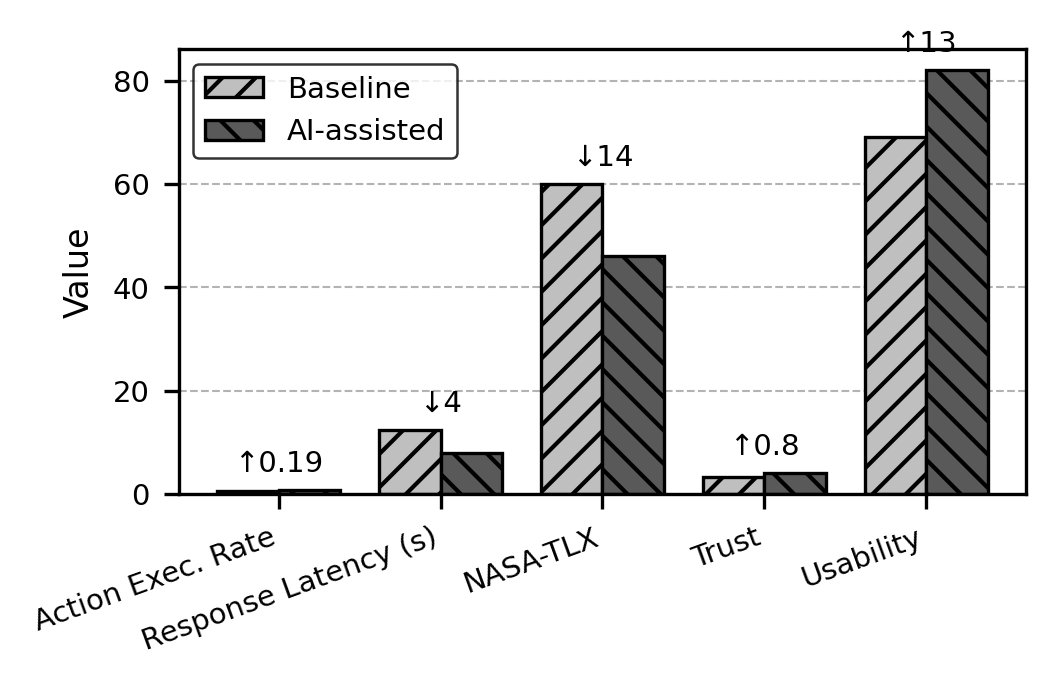
\includegraphics[width=0.9\linewidth]{fig_workload_trust_summary.png}
%DIFDELCMD <         \caption{Comparison of cognitive workload, trust, and usability between baseline and AI-assisted conditions. Lower NASA--TLX scores indicate reduced cognitive workload, while higher trust and usability scores indicate improved subjective evaluations.}
%DIFDELCMD <         \label{fig:workload_trust_summary}
%DIFDELCMD <     \end{figure}
%DIFDELCMD < %%%
\DIFdelend \DIFaddbegin \DIFadd{\textbf{Qualitative observations.}
    Post-task interviews were used to collect participants' comments on their experience. The comments were summarized into themes, but they were not systematically coded, and theme prevalence was not recorded. We therefore report them as informal observations that complement the quantitative results. We do not describe the study as a mixed-method evaluation.
}\DIFaddend 

    \DIFdelbegin \subsection{\DIFdel{Task Performance Outcomes}}
%DIFAUXCMD
\addtocounter{subsection}{-1}%DIFAUXCMD
%DIFDELCMD < 

%DIFDELCMD <     %%%
\DIFdel{The performance in the execution of }\DIFdelend \DIFaddbegin \subsection{\DIFadd{Statistical Analysis}}
    \DIFadd{All comparisons are within-subjects (baseline vs.\ AI-assisted, paired by participant) and used paired significance tests. H1 (AER) is }\DIFaddend the \DIFdelbegin \DIFdel{objective task was enhanced with the help of AI, as shown in Fig. ~\ref{fig:workload_trust_summary}}\DIFdelend \DIFaddbegin \DIFadd{primary hypothesis; H2--H4 concern secondary outcomes. For each outcome, we report the condition means (and SDs, where available) and the difference between conditions. For the outcomes with reported SDs (NASA--TLX, trust, SUS), we computed Cohen's $d_{av}$, i.e., the mean difference divided by the average of the two condition SDs \cite{Lakens2013}. Because $d_{av}$ does not take the within-subject correlation into account, it is not equivalent to $d_z$, the effect size on which the paired test is based. Exact test statistics, confidence intervals, assumption diagnostics, order-effect analyses, and multiplicity-corrected $p$-values could not be computed because the trial-level data were not available for re-analysis (Section~\ref{sec:lim_reporting}). The comparisons between escalated and non-escalated trials (Section~\ref{sec:res_escalation}) are descriptive only, because escalation is triggered by uncertainty or criticality and the two sets of trials are therefore not comparable.
}

    %DIF > ---------------------------------\input{./070-result}
    \section{\DIFadd{Results}}
    \DIFadd{Table~\ref{tab:primary} reports the primary and secondary outcomes. Interpretation follows in Section~\ref{sec:discussion}}\DIFaddend .

    \DIFdelbegin \DIFdel{It is observed that the rate of action execution was enhanced by a small amount, from 0.55 }\DIFdelend \DIFaddbegin \begin{table*}[t]
        \caption{Primary and Secondary Outcomes: Baseline vs.\ AI-Assisted (ACHDF), $n=52$, Within-Subjects}
        \label{tab:primary}
        \centering
        \begin{tabular}{l c c c c c}
            \toprule
            \textbf{Outcome} & \textbf{Baseline} & \textbf{AI-assisted} & \textbf{Difference} & \textbf{Paired test} & \textbf{Effect size} \\
            & M (SD) & M (SD) & (AI $-$ baseline) & & $d_{av}$ \\
            \midrule
            \multicolumn{6}{l}{\emph{Primary (H1)}} \\
            AER & 0.62 (n/a) & 0.81 (n/a) & $+0.19$ & $p < .01$ & n/a \\
            \midrule
            \multicolumn{6}{l}{\emph{Secondary (H2--H4)}} \\
            Response latency (s) & 12.4 (n/a) & 8.1 (n/a) & $-4.3$ & $p < .01$ & n/a \\
            NASA--TLX overall (0--100) & 59.8 (10.9) & 46.2 (9.6) & $-13.6$ & $p < .05$ & 1.32 \\
            Trust overall (1--5) & 3.4 (0.6) & 4.2 (0.5) & $+0.8$ & $p < .05$ & 1.45 \\
            SUS (0--100) & 68.5 (11.2) & 81.7 (9.4) & $+13.2$ & not reported & 1.28 \\
            \bottomrule
            \multicolumn{6}{p{0.92\linewidth}}{\footnotesize n/a: not available, because the trial-level data could not be re-analyzed. $p$-values are the significance thresholds of the original paired tests. Exact test statistics and 95\% confidence intervals could not be computed (Section~\ref{sec:lim_reporting}). $d_{av}$ = mean difference / average of the two condition SDs, computed from the reported means and SDs. It ignores the within-subject correlation and is not equivalent to the paired $d_z$. A single Cohen's $d$ of 0.86 given in the previous version could not be attributed to a specific outcome and has been removed.}
        \end{tabular}
    \end{table*}

    \subsection{\DIFadd{Action Execution and Response Latency}}
    \DIFadd{The mean AER was 0.62 }\DIFaddend in the baseline \DIFdelbegin \DIFdel{scenario to 0.74 }\DIFdelend \DIFaddbegin \DIFadd{condition and 0.81 }\DIFaddend in the AI-assisted \DIFdelbegin \DIFdel{scenario. This shows that the number of actions executed was higher in the AI-assisted scenario.
}%DIFDELCMD < 

%DIFDELCMD <     %%%
\DIFdel{It is also observed that the response time was reduced.
    The average response time was reduced from 12.3 seconds }\DIFdelend \DIFaddbegin \DIFadd{condition, a difference of 0.19 (paired test, $p < .01$).
    The mean response latency was 12.4~s }\DIFaddend in the baseline \DIFdelbegin \DIFdel{scenario to 8.0 seconds }\DIFdelend \DIFaddbegin \DIFadd{condition and 8.1~s }\DIFaddend in the AI-assisted \DIFdelbegin \DIFdel{scenario. The time was reduced by more than 4 seconds.This shows that the participants responded and executed actions in a better manner with the help of the AI system}\DIFdelend \DIFaddbegin \DIFadd{condition, a difference of 4.3~s (paired test, $p < .01$). Fig.~\ref{fig:latency_distribution} shows the latency distributions.
    Whether the difference in the AER arose mainly from fewer wrong actions or from fewer late actions could not be determined (Section~\ref{sec:lim_reporting})}\DIFaddend .

    \DIFdelbegin \subsection{\DIFdel{Cognitive Workload and Trust Outcomes}}
%DIFAUXCMD
\addtocounter{subsection}{-1}%DIFAUXCMD
\DIFdelend \DIFaddbegin \begin{figure}[t]
        \centering
        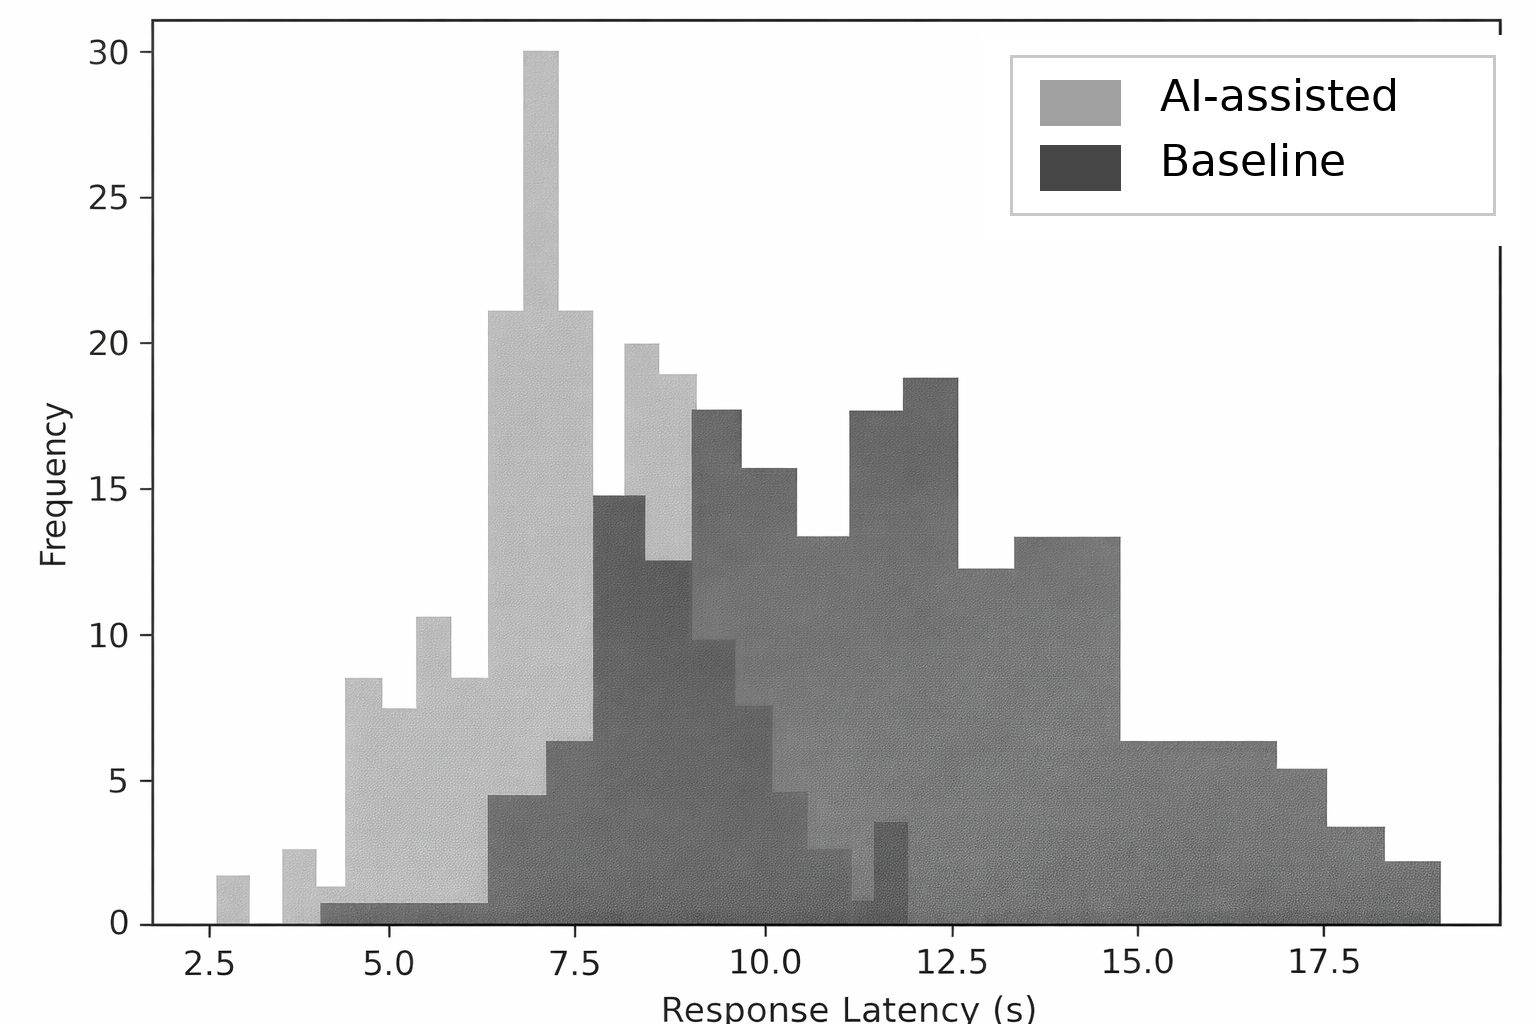
\includegraphics[width=0.9\linewidth]{fig_latency_distribution.png}
        \caption{Distribution of response latency under the baseline and AI-assisted conditions.}
        \label{fig:latency_distribution}
    \end{figure}
\DIFaddend 

    \DIFdelbegin \DIFdel{A graphical representation of the results for workload, trust, and usability is shown in }\DIFdelend \DIFaddbegin \subsection{\DIFadd{Workload, Trust, and Usability}}
    \DIFaddend Fig.~\ref{fig:workload_trust_summary} \DIFdelbegin \DIFdel{.
    Cognitive workload, as assessed by NASA--TLX, was significantly lower in the AI-assisted condition than in the baseline condition.
    The total score on the }\DIFdelend \DIFaddbegin \DIFadd{summarizes the subjective measures, and Table~\ref{tab:subscales} gives the subscale scores.
    The overall }\DIFaddend NASA--TLX \DIFdelbegin \DIFdel{assessment dropped from around 60 }\DIFdelend \DIFaddbegin \DIFadd{score was 59.8 (SD 10.9) }\DIFaddend in the baseline condition \DIFdelbegin \DIFdel{to 46 }\DIFdelend \DIFaddbegin \DIFadd{and 46.2 (SD 9.6) }\DIFaddend in the AI-assisted condition, a \DIFdelbegin \DIFdel{reduction of 14 points . This is a clear indication of reduced workload in the AI-assisted condition. The NASA--TLX scores are summarized in Table~\ref{tab:workload}.
    Trust ratings were higher for the AI-assisted system.
    The average }\DIFdelend \DIFaddbegin \DIFadd{difference of 13.6 points (paired test, $p < .05$; $d_{av} = 1.32$).
    The overall }\DIFaddend trust score was \DIFdelbegin \DIFdel{higher in the AI-assisted condition , increasing from around 3.2 in the }\DIFdelend \DIFaddbegin \DIFadd{3.4 (SD 0.6) in the }\DIFaddend baseline condition \DIFdelbegin \DIFdel{to 4.0 on a }\DIFdelend \DIFaddbegin \DIFadd{and 4.2 (SD 0.5) in the AI-assisted condition on the }\DIFaddend 5-point scale \DIFdelbegin \DIFdel{in the AI-assisted condition , indicating that the system was perceived as more trustworthy and appropriate in its guidance.
    Usability was also higher }\DIFdelend \DIFaddbegin \DIFadd{(paired test, $p < .05$; $d_{av} = 1.45$).
    The SUS score was 68.5 (SD 11.2) in the baseline condition and 81.7 (SD 9.4) }\DIFaddend in the AI-assisted condition \DIFdelbegin \DIFdel{. The system usability scores increased from around 69 to 82, a jump of 13 points, indicating that the participants found the AI-assisted system interface easier and more effective to use.
The trust and usability scores are summarized in Table~\ref{tab:trust_usability}.
}\DIFdelend \DIFaddbegin \DIFadd{($d_{av} = 1.28$). No significance test was reported for the SUS.
}\DIFaddend 

    \DIFdelbegin \subsection{\DIFdel{Effects of Uncertainty-Aware Escalation}}
    %DIFAUXCMD
\addtocounter{subsection}{-1}%DIFAUXCMD
\DIFdel{When the uncertainty thresholds were exceeded, human-in-the-loop escalation occurred. In such cases, the participants appropriately deferred their decisions until further confirmation or clarification was available. No increase in inappropriate use of the system recommendations in high-uncertainty cases was observed.
    The results comparing }\DIFdelend \DIFaddbegin \begin{figure}[t]
        \centering
        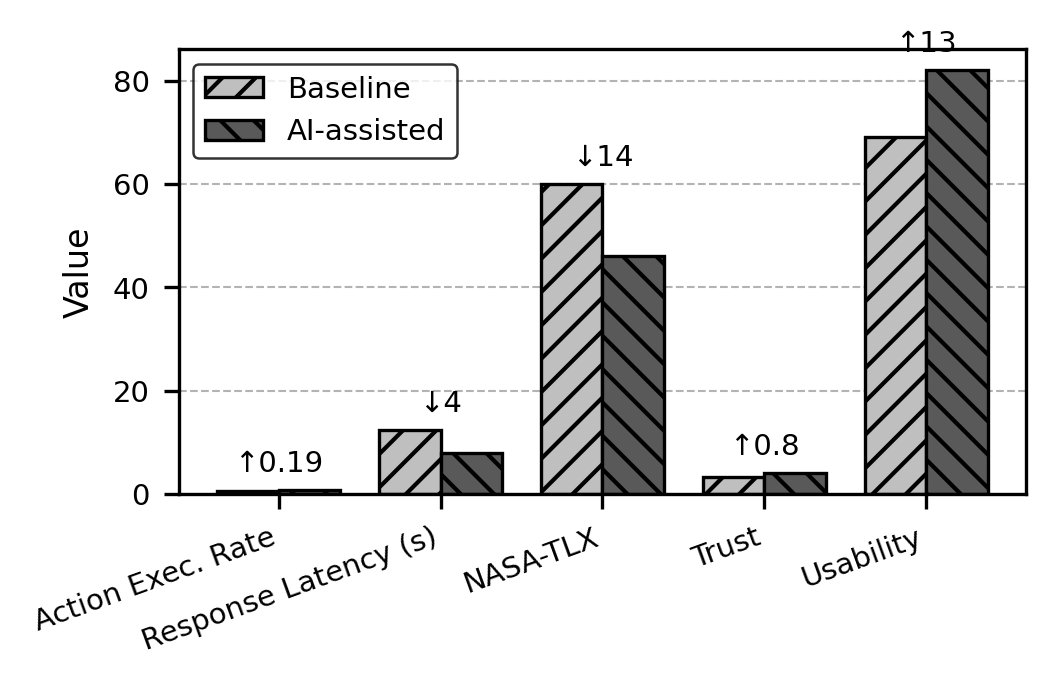
\includegraphics[width=0.9\linewidth]{fig_workload_trust_summary.png}
        \caption{Cognitive workload (NASA--TLX; lower is better), trust, and usability (higher is better) in the baseline and AI-assisted conditions.}
        \label{fig:workload_trust_summary}
    \end{figure}

    \begin{table}[t]
        \caption{Subscale Scores, M (SD)}
        \label{tab:subscales}
        \centering
        \begin{tabular}{lcc}
            \toprule
            \textbf{Subscale} & \textbf{Baseline} & \textbf{AI-assisted} \\
            \midrule
            \multicolumn{3}{l}{\emph{NASA--TLX (0--100)}} \\
            Mental demand & 63.4 (12.1) & 48.7 (10.5) \\
            Temporal demand & 58.9 (11.4) & 44.2 (9.8) \\
            Effort & 61.7 (13.0) & 49.1 (11.2) \\
            Frustration & 55.3 (14.6) & 41.8 (12.3) \\
            \midrule
            \multicolumn{3}{l}{\emph{Trust items (1--5)}} \\
            Perceived reliability & 3.2 (0.7) & 4.1 (0.6) \\
            Perceived predictability & 3.5 (0.8) & 4.2 (0.6) \\
            Perceived appropriateness & 3.4 (0.6) & 4.3 (0.5) \\
            \bottomrule
        \end{tabular}
    \end{table}

    \subsection{\DIFadd{Escalated and Non-Escalated Trials (Descriptive)}}
    \label{sec:res_escalation}
    \DIFadd{Table~\ref{tab:escalation} reports, descriptively, the rates of appropriate deferral and inappropriate reliance in }\DIFaddend escalated and non-escalated \DIFdelbegin \DIFdel{cases are presented in Table~\ref{tab:escalation}. These results show that uncertainty-aware escalation maintained system effectiveness while preventing over-reliance on the system. }\DIFdelend \DIFaddbegin \DIFadd{trials of the AI-assisted condition. Appropriate deferral denotes deferring the decision for further confirmation when the situation warranted it. Inappropriate reliance denotes following the AI recommendation when this was not appropriate. These two sets of trials are not equivalent conditions. Escalation is triggered by high uncertainty or criticality, and it explicitly prompts human review. The differences in Table~\ref{tab:escalation} therefore cannot be attributed causally to escalation. The number of trials in each set was not available.
}\DIFaddend 

    \DIFdelbegin \subsection{\DIFdel{Qualitative Observations}}
%DIFAUXCMD
\addtocounter{subsection}{-1}%DIFAUXCMD
\DIFdelend \DIFaddbegin \begin{table}[t]
        \caption{Behavior in Escalated vs.\ Non-Escalated Trials, AI-Assisted Condition (Descriptive)}
        \label{tab:escalation}
        \centering
        \begin{tabular}{lcc}
            \toprule
            \textbf{Metric} & \textbf{No escalation} & \textbf{Escalation triggered} \\
            \midrule
            Appropriate deferral rate & 0.21 & 0.47 \\
            Inappropriate reliance rate & 0.18 & 0.09 \\
            \bottomrule
        \end{tabular}
    \end{table}
\DIFaddend 

    \DIFdelbegin \DIFdel{The post-task interviews allowed for qualitative analysis of the participants' experiences. Participants often pointed out that the AI recommendations diminished the need for cross-referencing between different information sources. Some participants also emphasized the importance of having explicit uncertainty indicators to guide their confidence in decisions. Some qualitative findings are presented in }\DIFdelend \DIFaddbegin \subsection{\DIFadd{Qualitative Observations}}
    \DIFaddend Table~\ref{tab:qualitative} \DIFaddbegin \DIFadd{summarizes recurring comments from the post-task interviews. These are informal observations. They were not systematically coded, and their prevalence was not recorded (Section~\ref{sec:measures})}\DIFaddend .
\DIFdelbegin \DIFdel{These findings supplement the quantitative findings by providing a glimpse into the participants' experiences with the system during decision-making tasks. To mitigate the potential for a Type~I error due to multiple comparisons, all primary hypotheses were defined a~priori, and consistent performance patterns were verified across different objective and subjective measures.
}%DIFDELCMD < 

%DIFDELCMD <     \begin{table}[t]
%DIFDELCMD <         \caption{Cognitive Workload and Trust Scores}
%DIFDELCMD <         \label{tab:workload_trust}
%DIFDELCMD <         \centering
%DIFDELCMD <         \begin{tabular}{l c c}
%DIFDELCMD <             \hline
%DIFDELCMD <             Measure & Baseline & AI-Assisted \\
%DIFDELCMD <             \hline
%DIFDELCMD <             NASA--TLX & 59.8 & 46.2 \\
%DIFDELCMD <             Trust score & 3.4 & 4.2 \\
%DIFDELCMD <             \hline
%DIFDELCMD <         \end{tabular}
%DIFDELCMD <     \end{table}
%DIFDELCMD < %%%
\DIFdelend 

    \DIFdelbegin %DIFDELCMD < \begin{table}[t]
%DIFDELCMD <         \caption{Action execution and response latency (controlled study)}
%DIFDELCMD <         \label{tab:action_latency}
%DIFDELCMD <         \centering
%DIFDELCMD <         \begin{tabular}{lcc}
%DIFDELCMD <             \toprule
%DIFDELCMD <             \textbf{Metric} & \textbf{Baseline} & \textbf{AI-assisted} \\
%DIFDELCMD <             \midrule
%DIFDELCMD <             Action Execution Rate (AER) & 0.62 & 0.81 \\
%DIFDELCMD <             Response Latency (s) & 12.4 & 8.1 \\
%DIFDELCMD <             Effect size (Cohen's $d$) & \multicolumn{2}{c}{0.86} \\
%DIFDELCMD <             \bottomrule
%DIFDELCMD <         \end{tabular}
%DIFDELCMD <     \end{table}
%DIFDELCMD < 

%DIFDELCMD <     \begin{table}[t]
%DIFDELCMD <         \caption{Workload, trust, and usability outcomes (controlled study)}
%DIFDELCMD <         \label{tab:workload_trust}
%DIFDELCMD <         \centering
%DIFDELCMD <         \begin{tabular}{lcc}
%DIFDELCMD <             \toprule
%DIFDELCMD <             \textbf{Metric} & \textbf{Baseline} & \textbf{AI-assisted} \\
%DIFDELCMD <             \midrule
%DIFDELCMD <             NASA--TLX (overall) & 59.8 & 46.2 \\
%DIFDELCMD <             Trust (Likert-type composite) & 3.4 & 4.2 \\
%DIFDELCMD <             Usability score & 68.5 & 81.7 \\
%DIFDELCMD <             \bottomrule
%DIFDELCMD <         \end{tabular}
%DIFDELCMD <     \end{table}
%DIFDELCMD < 

%DIFDELCMD <     \begin{table}[t]
%DIFDELCMD <         \caption{Outcomes by uncertainty-aware escalation status}
%DIFDELCMD <         \label{tab:escalation}
%DIFDELCMD <         \centering
%DIFDELCMD <         \begin{tabular}{lcc}
%DIFDELCMD <             \toprule
%DIFDELCMD <             \textbf{Metric} & \textbf{No escalation} & \textbf{Escalation triggered} \\
%DIFDELCMD <             \midrule
%DIFDELCMD <             Appropriate deferral rate & 0.21 & 0.47 \\
%DIFDELCMD <             Inappropriate reliance rate & 0.18 & 0.09 \\
%DIFDELCMD <             \bottomrule
%DIFDELCMD <         \end{tabular}
%DIFDELCMD <     \end{table}
%DIFDELCMD < %%%
\DIFdelend \DIFaddbegin \begin{table}[t]
        \caption{Informal Observations From Post-Task Interviews (Not Systematically Coded)}
        \label{tab:qualitative}
        \centering
        \begin{tabular}{p{0.30\linewidth}p{0.60\linewidth}}
            \toprule
            \textbf{Theme} & \textbf{Observation (paraphrased)} \\
            \midrule
            Reduced context switching & Recommendations reduced the need to cross-reference multiple sources. \\
            Usefulness of uncertainty cues & Participants used uncertainty cues to decide when to defer or seek confirmation. \\
            Accountability and control & The ability to override improved perceived safety and responsibility. \\
            \bottomrule
        \end{tabular}
    \end{table}
\DIFaddend 

    \DIFdelbegin %DIFDELCMD < \begin{table}[t]
%DIFDELCMD <         \caption{Qualitative themes from post-task interviews}
%DIFDELCMD <         \label{tab:qualitative}
%DIFDELCMD <         \centering
%DIFDELCMD <         \begin{tabular}{p{0.27\linewidth}p{0.64\linewidth}}
%DIFDELCMD <             \toprule
%DIFDELCMD <             \textbf{Theme} & \textbf{Illustrative observation (paraphrased)} \\
%DIFDELCMD <             \midrule
%DIFDELCMD <             Reduced context switching & Recommendations decreased the need to cross-reference multiple sources. \\
%DIFDELCMD <             Uncertainty cue usefulness & Participants used uncertainty cues to decide when to defer or seek confirmation. \\
%DIFDELCMD <             Accountability and control & Human override improved perceived safety and responsibility. \\
%DIFDELCMD <             \bottomrule
%DIFDELCMD <         \end{tabular}
%DIFDELCMD <     \end{table}
%DIFDELCMD < %%%
\DIFdelend %DIF > ----------------------------------------\input{./080-discussion}
\DIFaddbegin \section{\DIFadd{Discussion}}
\label{sec:discussion}
\DIFadd{This section interprets the results from a human--machine systems perspective. In line with the JCS view \cite{Hollnagel2005JCS,Woods2006JCS}, we interpret the results at the level of the joint human--AI system. Because the AI-assisted condition differed from the baseline in several features at once, the interpretations below about \emph{which} features produced the effects are hypotheses, not demonstrated causal pathways.
}\DIFaddend 

\DIFdelbegin \subsection{\DIFdel{Mechanism and Multi-layer Analysis Under ACHDF}}
    %DIFAUXCMD
\addtocounter{subsection}{-1}%DIFAUXCMD
%DIFDELCMD < \label{sec:results_mechanism}
%DIFDELCMD < %%%
\DIFdelend \DIFaddbegin \subsection{\DIFadd{Action Execution in the Joint Human--AI System}}
\DIFadd{In the AI-assisted condition, the AER was higher and response latency shorter than with the dashboard. This is consistent with H1 and H2. Evaluating the system by action execution, rather than by prediction accuracy, follows directly from the JCS perspective. In AI decision-support research, however, evaluation is still dominated by accuracy and information quality \cite{Lai2023FAccT,Muller2022CHIWORK,Yang2022THMSReview}. Our results illustrate that what a human--AI system achieves depends on how support is structured to lead to action, not only on whether support is available.
}\DIFaddend 

\DIFdelbegin \DIFdel{In order to provide a structured understanding of how the achieved results were obtained at the behavioral level, we also analyzed the results through the prism of the Action-Centered Human--AI Decision Framework (ACHDF). This analysis does not include any new outcome measures but structures the existing results to reveal multi-layered patterns relevant to human action in the context of uncertainty.
From the mechanism perspective, the increase in Action Execution Rate and the reduction in response latency (Table~\ref{tab:action_latency}, Fig.~\ref{fig:latency_distribution}) may be considered a behavioral outcome of uncertainty-aware function allocation, where the representation of uncertainty directly influences the allocation of decisions to the AI or human operators in terms of timing and correctness of action execution. At the level of error structure, uncertainty-aware escalation was found to influence participants’ responses in high-uncertainty scenarios. As depicted in Table~\ref{tab:escalation}, escalation was linked to increased appropriate deferral and reduced inappropriate reliance. These results indicate that uncertainty-aware escalation selectively mitigated failure modes related to hesitation and over-reliance, rather than indiscriminately increasing reliance on automation.
Lastly, qualitative results (Table~\ref{tab:qualitative}) and reductions in workload (Table~\ref{tab:workload}) indicate changes in decision processes in }\DIFdelend \DIFaddbegin \DIFadd{Several features of }\DIFaddend the AI-assisted condition \DIFdelbegin \DIFdel{. Participants’ self-reported context switching and decision transitions align with reductions in response latency and workload. These findings on all three levels align with the premise of ACHDF: that human action in uncertain situations can be explained by the interaction of uncertainty-aware risk representation, bounded autonomy, calibrated trust, and cognitive workload management. Moreover, statistical tests for comparing the baseline and AI-assisted conditions revealed that the improvement in the rate of action execution and the reduction of latency while responding were statistically significant at a $p$ value of less than 0.01. Differences observed for cognitive workload and trust levels, as measured by the NASA--TLX scale, were statistically significant at a $p$ value of less than 0.05}\DIFdelend \DIFaddbegin \DIFadd{could explain the improvement: the presence of a recommendation, its action-oriented phrasing, the explicit uncertainty and criticality cues, and escalation. Our design does not separate these features. In particular, we cannot conclude that presenting recommendations in an action format, rather than a risk format, caused the improvement. A factorial design that varies the format while holding the other features constant is needed to test this (Section~\ref{sec:limitations}). Because the AER could not be decomposed, it also remains open whether the improvement came mainly from fewer wrong actions or from fewer late actions (Section~\ref{sec:lim_reporting})}\DIFaddend .

%DIF < ----------------------------------------\input{./080-discussion}
\DIFdelbegin \section{\DIFdel{Discussion}}
%DIFAUXCMD
\addtocounter{section}{-1}%DIFAUXCMD
\DIFdel{This section interprets the empirical findings from a human--machine systems perspective and situates them within the broader literature on human--AI decision making. Rather than focusing on application-specific results, }\DIFdelend \DIFaddbegin \subsection{\DIFadd{Framework-Based Interpretation of }\DIFaddend the \DIFdelbegin \DIFdel{discussion emphasizes generalizable insights for the design and evaluation of human--AI decision systems operating under uncertainty \cite{Bach2024Access,PerezCerrolaza2024CSUR,Lai2023FAccT,Yang2022THMSReview}. In particular, this work contributes to the core concerns of \textit{Human--Machine Systems} by explicitly linking }\DIFdelend \DIFaddbegin \DIFadd{Results}}
\label{sec:interpretation}
\DIFadd{The following interpretation organizes the observed results along the ACHDF layers. It does not test the proposed mechanisms; it is a framework-based reading of the existing outcomes.
\emph{Action level:} the higher AER and lower latency (Table~\ref{tab:primary}) are consistent with the idea that }\DIFaddend uncertainty-aware \DIFdelbegin \DIFdel{function allocation to observable human action execution. By doing so, it extends classic HMS constructs---such as trust calibration, workload, and authority allocation---from internal cognitive or perceptual states to measurable behavioral outcomes}\DIFdelend \DIFaddbegin \DIFadd{adaptation of support helps operators move from risk interpretation to action}\DIFaddend .
\DIFaddbegin \DIFadd{\emph{Error-structure level:} in escalated trials, appropriate deferral was more frequent and inappropriate reliance less frequent than in non-escalated trials (Table~\ref{tab:escalation}). Because escalation is triggered by uncertainty and criticality and itself prompts human review, this pattern is descriptive. It is compatible with, but does not demonstrate, a protective effect of escalation against over-reliance.
\emph{Process level:} interview themes on reduced context switching (Table~\ref{tab:qualitative}) and lower NASA--TLX scores (Table~\ref{tab:subscales}) suggest that the AI-assisted condition changed the decision process.
}\DIFaddend 

\DIFdelbegin %DIFDELCMD < \subsection{%%%
\DIFdel{Implications for Human--AI Decision Systems}%DIFDELCMD < \MBLOCKRIGHTBRACE
%DIFDELCMD < %%%
\DIFdel{The results show that human performance gain is not simply a function of the availability of AI support, but also depends on how that support is organized to guide human actionexecution.
By directly assessing action execution as an outcome measure, this research extends previous research that primarily tested decision support systems in terms of the accuracy of predictions or the quality of information \cite{Lai2023FAccT,Muller2022CHIWORK,Yang2022THMSReview}. From a human--machine system perspective, action execution is the end result of human information processing that combines elements of perception, understanding, trust, and workload into system performance \cite{Hodgson2013THMS,Bach2024Access}.
The increase in Action Execution Rate and the decrease in response latency indicate that human--AI systems are capable of significantly influencing human behavior when recommendations are presented in action format instead of risk format. This supports the move towards an outcome-oriented human--machine system research area where the effectiveness of AI support is determined in terms of human action instead of computer performance \cite{Lai2023FAccT,Yang2022THMSReview}.
This research contributes to the Human--Machine Systems area by empirically connecting function allocation with uncertainty to human }\DIFdelend \DIFaddbegin \DIFadd{\textbf{Workload as a possible explanation.} Lower workload is a plausible contributor to better }\DIFaddend action execution. The \DIFdelbegin \DIFdel{results demonstrate how design decisions in the architecture (bounded autonomy, uncertainty representation, and escalation strategies) map to behavioral phenomena, thus closing the theoretical-practice divide in human factors theory and human--AI system design \cite{Bach2024Access,Assaad2023TAS,Zhang2022THMS}.
In this respect, the Action-Centered Human--AI Decision Framework (ACHDF)may also be used as an analytical tool for identifying failure modes in existing human--AI systems, aside from the system examined in this research \cite{Yang2022THMSReview,Lai2023FAccT}}\DIFdelend \DIFaddbegin \DIFadd{NASA--TLX, however, is a retrospective, subjective, condition-level measure, and we did not test whether the reduction in workload explains the improvement in AER (e.g., with a mediation analysis). This link should therefore be regarded as a possible explanatory mechanism, not a demonstrated pathway}\DIFaddend .

\subsection{Trust \DIFdelbegin \DIFdel{Calibration }\DIFdelend and Automation Bias}
\DIFdelbegin \DIFdel{The main contribution of this research is in the way it approaches the issue of trust calibration. The findings show that the more trust participants had }\DIFdelend \DIFaddbegin \DIFadd{Perceived trust was higher }\DIFaddend in the AI-assisted \DIFdelbegin \DIFdel{system, the more this did not translate to automation bias. Instead, participants displayed appropriate trust in the system and delayed action in situations of high uncertainty and appropriate use of human-in-the-loop escalation mechanisms \cite{Raji2019AIES,Raji2022CACM,Weidinger2022FAccT}. The findings demonstrate the effect of uncertainty-aware design and the use of design constraints in avoiding typical automation failure modes. In this way, the system did not provide false confidence to the participants. These findings validate human factors theories emphasizing the importance of trust calibration in effective human--AI cooperation and provide evidence of this in design \cite{Hodgson2013THMS,Bach2024Access}. These results provide empirical support for long-held theoretical assertions in human--machine systems research that }\DIFdelend \DIFaddbegin \DIFadd{condition. Higher trust is not the same as \emph{calibrated} trust. Calibration requires that reliance matches the actual reliability of the advice \cite{Lee2004}. Showing calibration would require relating trust or reliance to the correctness of the AI's recommendations, trial by trial. The greater deferral in escalated trials is also not evidence of calibration, because escalation itself prompts human review. We therefore make no claim that ACHDF calibrates trust.
}

\DIFadd{Similarly, }\DIFaddend automation bias can be \DIFdelbegin \DIFdel{reduced by incorporating uncertainty representation and human-in-the-loop escalation. Contrary to the potential for increasing over-reliance, the proposed design facilitated calibrated trust by aligning perceived system confidence with actual uncertainty \cite{Miller2019XRDS,Weidinger2022FAccT,Lai2023FAccT}}\DIFdelend \DIFaddbegin \DIFadd{directly assessed only on trials in which the AI's advice is wrong, by measuring how often participants accept it \cite{Parasuraman2010}. The study did not analyze behavior on trials with erroneous AI recommendations, so it cannot show whether ACHDF reduces automation bias. This is an important topic for future work}\DIFaddend .

\DIFdelbegin %DIFDELCMD < \begin{table}[t]
%DIFDELCMD <         \caption{Design Implications for Human--AI Decision Systems}
%DIFDELCMD <         \label{tab:design_implications}
%DIFDELCMD <         \centering
%DIFDELCMD <         \begin{tabular}{l l}
%DIFDELCMD <             \hline
%DIFDELCMD <             Finding & Design Implication \\
%DIFDELCMD <             \hline
%DIFDELCMD <             Higher AER & Action-oriented recommendations \\
%DIFDELCMD <             Reduced workload & Information structuring \\
%DIFDELCMD <             Calibrated trust & Explicit uncertainty \\
%DIFDELCMD <             \hline
%DIFDELCMD <         \end{tabular}
%DIFDELCMD <     \end{table}
%DIFDELCMD <     

%DIFDELCMD < %%%
\DIFdelend \subsection{\DIFdelbegin \DIFdel{Design Implications for High-Risk Domains}\DIFdelend \DIFaddbegin \DIFadd{Ecological Validity of Escalation}\DIFaddend }
\DIFdelbegin \DIFdel{Although the empirical studywas carried out in the context of disaster response, the design principles and results can be generalized to other high-risk domains such as healthcare, transportation, and industrial safety, where the cost of inappropriate or delayed response is high, and complete automation is not always feasible or desirable \cite{PerezCerrolaza2024CSUR,Rao2024IJDRS,Rokhideh2025IJDRS,Birkmann2013NatHazards}. Similar action-centered constraints and explainability considerations also arise in cyber-physical production and Industry~4.0 security decision support \cite{Farhan2025TCE}.
The findings of the study indicate }\DIFdelend \DIFaddbegin \DIFadd{In the study, participants could defer a decision when the system escalated. In real time-critical emergencies, deferral may not be feasible or may itself be costly: an operator may have to act on uncertain information before an evacuation window closes. The lower inappropriate reliance observed in escalated trials may therefore not carry over to settings where deferral is constrained, and forced action under uncertainty might change both reliance and workload. Future studies should assign explicit costs to deferral and include forced-choice conditions.
}

    \begin{table}[t]
        \caption{Observed Findings and Candidate Design Implications (to Be Tested Component-Wise)}
        \label{tab:design_implications}
        \centering
        \begin{tabular}{p{0.38\linewidth} p{0.52\linewidth}}
            \toprule
            Observed finding & Candidate design implication \\
            \midrule
            Higher AER, lower latency & Action-oriented recommendations \\
            Lower NASA--TLX & Consolidated information structuring \\
            Higher perceived trust & Explicit uncertainty and criticality cues \\
            \bottomrule
        \end{tabular}
    \end{table}

\subsection{\DIFadd{Design Implications}}
\DIFadd{Within the scope of the evaluated task, the results suggest }\DIFaddend that human--AI \DIFdelbegin \DIFdel{decision-making systems should be designed in such a way that they }\DIFdelend \DIFaddbegin \DIFadd{decision support systems may benefit from }\DIFaddend (1) \DIFdelbegin \DIFdel{model }\DIFdelend \DIFaddbegin \DIFadd{representing }\DIFaddend uncertainty explicitly, (2) \DIFdelbegin \DIFdel{provide }\DIFdelend \DIFaddbegin \DIFadd{providing }\DIFaddend action guidance rather than \DIFaddbegin \DIFadd{only }\DIFaddend passive information display, and (3) \DIFdelbegin \DIFdel{allocate decision authority dynamically }\DIFdelend \DIFaddbegin \DIFadd{adapting the level and form of support to uncertainty and criticality }\DIFaddend through human-in-the-loop escalation\DIFdelbegin \DIFdel{\cite{Assaad2023TAS,Zhang2022THMS,Bach2024Access}. Based on the Human--Machine Systems model, the results of the current study imply that effective decision systems with AI assistance need to be based on the concepts of bounded autonomy and decision authority allocation, as well as uncertainty-aware interaction. These concepts are not limited to the disaster response domain and are generally applicable to a wide variety of safety-critical human--machine systems with AI assistance \cite{Yang2022THMSReview,PerezCerrolaza2024CSUR}. The observed effects of the described phenomenon are not domain-specific but rather general mechanisms of human--machine interaction, which are relevant to any }\DIFdelend \DIFaddbegin \DIFadd{, while leaving final authority with the human \cite{Assaad2023TAS,Zhang2022THMS,Bach2024Access,Parasuraman2000LOA}. Table~\ref{tab:design_implications} lists these candidate implications. Because the components were not manipulated separately, each implication should be tested individually. Whether they transfer to other }\DIFaddend safety-critical \DIFdelbegin \DIFdel{decision system \cite{Bach2024Access,Hodgson2013THMS}.In general, the current study contributes to the broader area of human--machine systems by showing the benefits of the application of human-centered AI decision systems with awareness of uncertainty for the execution of actions without compromising safety and accountability \cite{Lai2023FAccT,Yang2022THMSReview}. The design implications that are critical based on the findings are presented in Table~\ref{tab:design_implications}. In providing insight into the manner in which architectural design translates into behavioral outcomes, the results contribute to the domain of human machine systems with respect to trust calibration and cognitive ergonomics. }\DIFdelend \DIFaddbegin \DIFadd{domains, such as healthcare, transportation, and industrial safety \cite{PerezCerrolaza2024CSUR,Farhan2025TCE}, has not been tested here (Table~\ref{tab:achdf_transferability}).
}\DIFaddend 

    %---------------------------------\input{./090-futurework}
    \section{Limitations and Future Work}
    \DIFdelbegin \DIFdel{The research has several limitations, which also point to potential directions for future research in similar studies. Although the research provides valuable data in terms of the effectiveness of the human--AI system in decision-making, it must be considered in relation to the limitations of this research.
        }\DIFdelend \DIFaddbegin \label{sec:limitations}
\DIFaddend 

    \DIFdelbegin \subsection{\DIFdel{Generalization}}
    %DIFAUXCMD
\addtocounter{subsection}{-1}%DIFAUXCMD
\DIFdel{The study has conducted an empirical evaluation using a set of decision scenarios in relation to a disaster response scenario. Although this scenario is representative of a high-stakes decision-making scenario in which there is considerable uncertainty }\DIFdelend \DIFaddbegin \subsection{\DIFadd{Bundled Intervention}}
    \DIFadd{The AI-assisted condition differed from the baseline in several features at once. The study therefore estimates the effect of the integrated ACHDF configuration and cannot attribute effects to individual components (uncertainty display, action format, escalation, guardrails). Future work should use factorial or ablation designs.
}

    \subsection{\DIFadd{Trust Calibration and Automation Bias}}
    \DIFadd{Trust was measured as a self-reported attitude at the condition level, and behavior on trials with erroneous AI recommendations was not analyzed. Hence, neither calibration nor automation bias could be assessed directly. Future studies should include trials with incorrect advice and measure reliance trial by trial.
}

    \subsection{\DIFadd{Domain and Population Generalizability}}
    \DIFadd{The evaluation was conducted only with disaster-response scenarios in a simulated setting. Participants were not required to have domain expertise, and the sample was not composed specifically of emergency-management professionals. Trained emergency operators may behave differently: they may rely less on recommendations, use different heuristics, or experience different workload. Generalization to other domains (e.g.}\DIFaddend , \DIFdelbegin \DIFdel{future research can be conducted to evaluate the generalization of }\DIFdelend \DIFaddbegin \DIFadd{medical triage, autonomous driving supervision, traffic management) and to professional operators remains future work. The ecological limits of deferral (Section~\ref{sec:discussion}) also belong here.
}

    \subsection{\DIFadd{Reporting and Analysis Limitations}}
    \label{sec:lim_reporting}
    \DIFadd{Several analyses and details requested for a complete account of the study could not be provided, because the trial-level data and some study materials were not available for re-analysis. The affected results should be interpreted with corresponding caution:
    }\begin{itemize}
        \item \DIFadd{\emph{Inferential statistics.} Only the significance thresholds of the original paired tests are available. Exact test statistics, 95\% confidence intervals, assumption diagnostics, the paired effect size $d_z$, order-effect analyses, and multiplicity-corrected $p$-values could not be computed. SDs for the AER and response latency are not available, and the paired test used for each outcome is not documented. No a priori power analysis was reported; the sensitivity analysis (Section~\ref{sec:participants}) indicates adequate power only for effects of about $d_z \geq 0.40$.
        }\item \DIFadd{\emph{AER construction.} The procedure for defining the appropriate action and the length of the time window are not documented in detail, and the AER could not be decomposed into action correctness and timeliness. Consequently, it cannot be determined whether execution failures were due to wrong actions or to delays.
        }\item \DIFadd{\emph{Task and materials.} The number and composition of scenarios (by uncertainty and criticality), }\DIFaddend the \DIFdelbegin \DIFdel{proposed design principles across diverse domains and professionals in which there is considerable expertise. }\DIFdelend \DIFaddbegin \DIFadd{full set of response options, the per-trial time limit, the matching of scenario difficulty, the training content and any pass criterion, and interface screenshots are not reported. This limits reproducibility.
        }\item \DIFadd{\emph{System implementation.} The risk model's estimation and calibration procedure, the criticality scale and thresholds, and the specific guardrail rules are not reported. The evaluation therefore concerns the interaction design as experienced by participants, not the validity of these components.
        }\item \DIFadd{\emph{Measures.} The trust items have no published validation and their internal consistency could not be estimated. The interview data were not systematically coded. The number of escalated trials is not available.
    }\end{itemize}
    \DIFadd{Future studies should preregister their analyses and share trial-level data and materials so that these analyses can be reported in full.
}\DIFaddend 

    \DIFdelbegin \subsection{\DIFdel{Long-Term Trust Effects}}
    %DIFAUXCMD
\addtocounter{subsection}{-1}%DIFAUXCMD
\DIFdel{The research has focused on the }\DIFdelend \DIFaddbegin \subsection{\DIFadd{Long-Term Trust Effects}}
    \DIFadd{The study captured only }\DIFaddend short-term \DIFdelbegin \DIFdel{effects of human--AI systems. Although it is recognized that the study has focused on the short term, it is anticipated that the long-term effects of trust will be considerable in relation to operators' exposure to the system and its behavior in relation to uncertainty escalation. }%DIFDELCMD < 

%DIFDELCMD <     %%%
\subsection{\DIFdel{Extension of the Research Beyond Disaster Response}}
    %DIFAUXCMD
\addtocounter{subsection}{-1}%DIFAUXCMD
\DIFdel{The research has focused on the domain of disaster response and has recognized this domain as effective in relation to testing systems in a high-stakes scenario.
Although the domain is recognized as effective in relation to testing systems in a high-stakes scenario, future research can be conducted to extend the system beyond this domain to other high-stakes domains such as medical systems and traffic management systems}\DIFdelend \DIFaddbegin \DIFadd{effects within a single session. Trust and reliance may change with longer exposure to the system and to its escalation behavior, which calls for longitudinal field studies}\DIFaddend .

    %-------------------------------\input{./092-conclusion}
\section{Conclusion}
This \DIFdelbegin \DIFdel{work evaluated }\DIFdelend \DIFaddbegin \DIFadd{paper presented ACHDF, }\DIFaddend an action-centered human--AI decision \DIFdelbegin \DIFdel{system for disaster-risk contexts and showed that an ACHDF-based, uncertainty-aware architecture improves action execution (higher AER and lower response latency) while reducing cognitive workload (NASA--TLX) and supporting calibrated trust without increasing automation bias. By empirically linking }\DIFdelend \DIFaddbegin \DIFadd{framework that instantiates the joint cognitive systems perspective for disaster-response decision support. ACHDF combines }\DIFaddend uncertainty-aware \DIFdelbegin \DIFdel{function allocation}\DIFdelend \DIFaddbegin \DIFadd{risk estimation}\DIFaddend , guardrailed recommendations, and \DIFdelbegin \DIFdel{human-in-the-loop escalationto observable action execution , the paper advances core concerns of human--machine systems and provides transferable }\DIFdelend \DIFaddbegin \DIFadd{uncertainty- and criticality-triggered escalation, while the human keeps final decision authority. In a within-subjects study with 52 participants, the integrated ACHDF configuration, compared with a conventional dashboard, was associated with a higher action execution rate, shorter response latency, lower self-reported workload, and higher perceived trust and usability. The study did not isolate individual components, assess trust calibration or automation bias directly, or test other domains or professional operators. These questions define the next steps toward validated }\DIFaddend design principles for \DIFdelbegin \DIFdel{other safety-critical decision ecologies}\DIFdelend \DIFaddbegin \DIFadd{human--AI decision support under uncertainty}\DIFaddend .

\section*{Acknowledgment}
The author thanks the \DIFdelbegin \DIFdel{municipal partners who supported the pilot deployment and the }\DIFdelend study participants for their time and insights\DIFdelbegin \DIFdel{. The author thanks the colleagues in the areas of human machine }\DIFdelend \DIFaddbegin \DIFadd{, and colleagues in human--machine }\DIFaddend systems and human-centered AI research for \DIFdelbegin \DIFdel{the valuable discussionsthat contributed to the development of this work}\DIFdelend \DIFaddbegin \DIFadd{valuable discussions}\DIFaddend .




%% How to support DOI (Digital Obect Identifier) in reference section:
% \url{https://ctan.org/tex-archive/macros/latex/contrib/IEEEtran/bibtex?lang=en}
% \url{https://people.kth.se/~maguire/myIEEEtran.bst}
% \url{https://ipfs-sec.stackexchange.cloudflare-ipfs.com/tex/A/question/67444.html}
% \url{https://ipfs-sec.stackexchange.cloudflare-ipfs.com/tex/A/question/394811.html}
\bibliographystyle{IEEEtranDOI}

%% Type1: sorting, keep sequence of reference numbers that user typed.
%\bibliographystyle{IEEEtranDOI} 

%% Type2: sorting, re-arrange sequence of reference numbers that user typed
% for ascending cite number.
% \bibliographystyle{IEEEtranDOI}

%% Add reference papers
\bibliography{reference-data}



% omitting for THMS journal
% 


% === Author Biographies ===
\vspace{2em} % (필요 시 조절)
\noindent
\begin{minipage}{\linewidth}
\begin{IEEEbiography}[{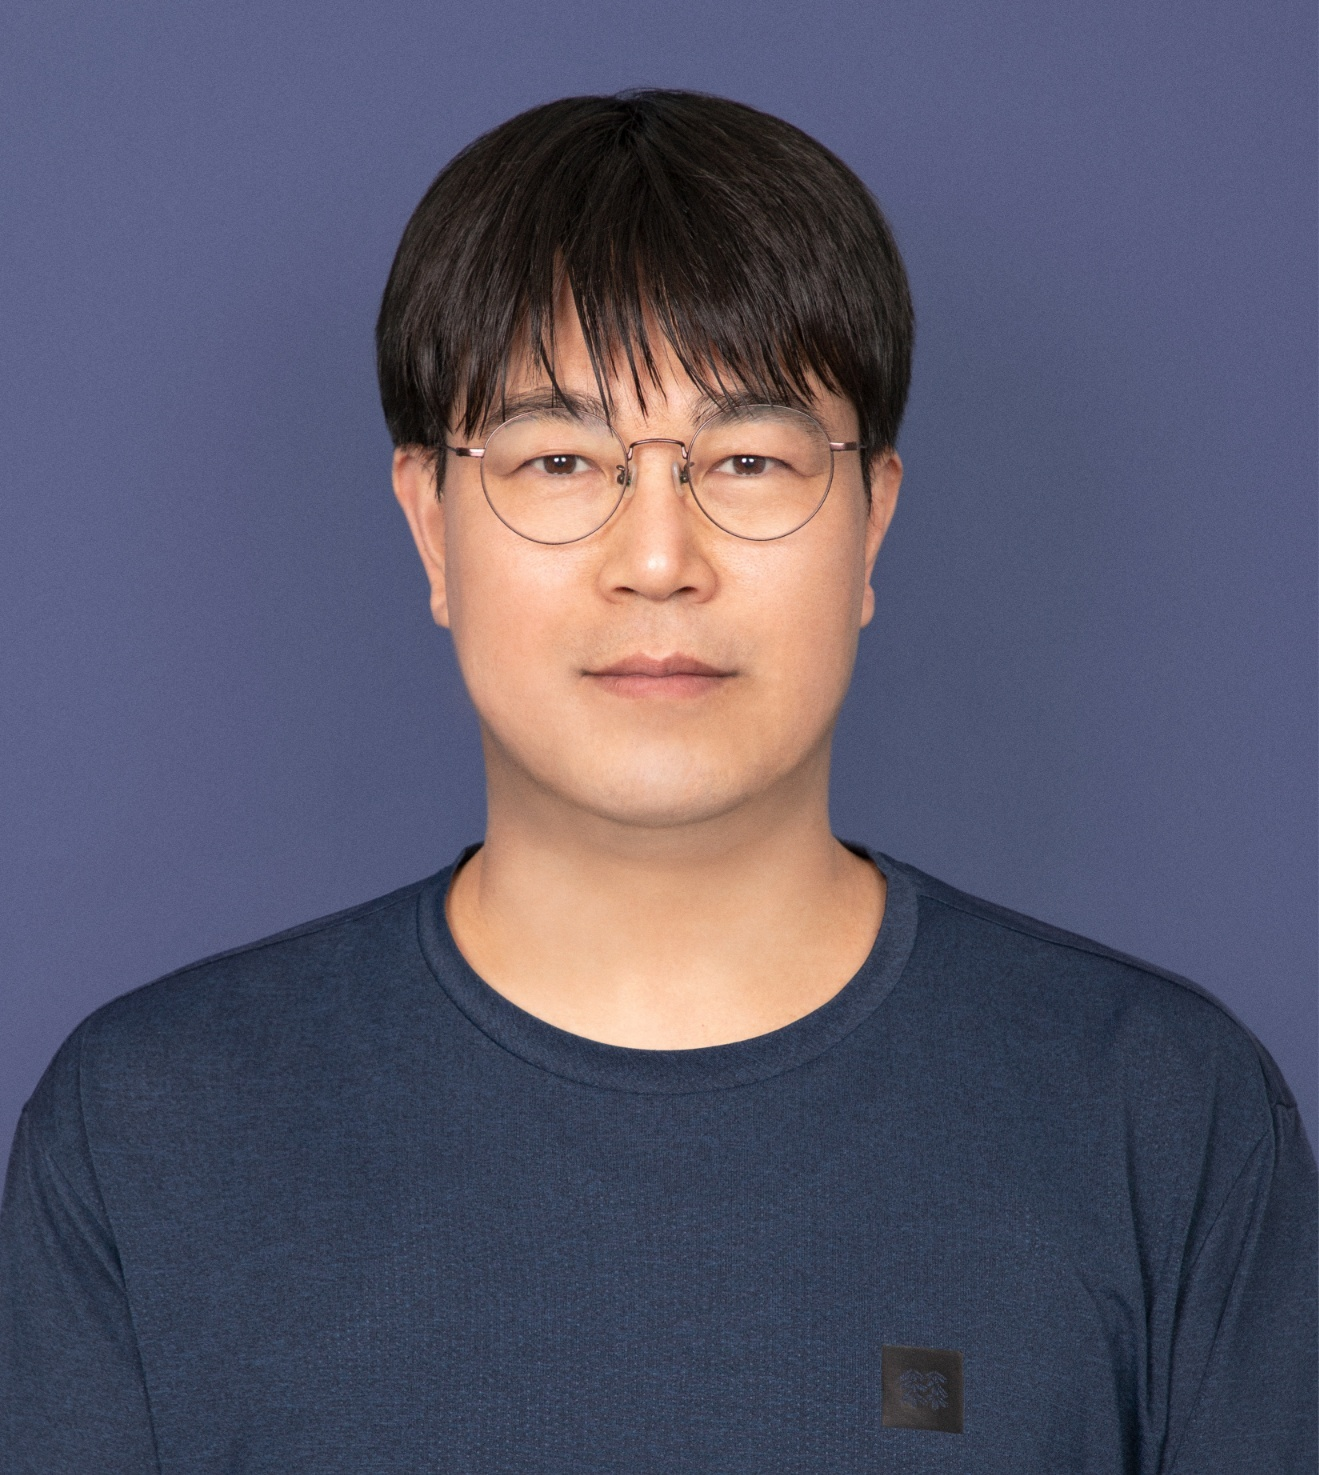
\includegraphics[width=1in,height=1.25in,clip,keepaspectratio]{./fig_author-lim2.png}}]{Geunsik Lim}
received the B.S. degree in Computer Science and Engineering from Ajou University, South Korea, in 2003, and the M.S. and Ph.D. degrees in Electrical and Computer Engineering from Sungkyunkwan University, South Korea, in 2014 and 2023, respectively. He is currently a principal software engineer at Samsung Electronics in South Korea. His research interests include system optimization, operating systems, software platforms, and on-device artificial intelligence. 
\end{IEEEbiography}
\end{minipage}


\end{document}
